\documentclass[conference]{IEEEtran}
\IEEEoverridecommandlockouts
% The preceding line is only needed to identify funding in the first footnote. If that is unneeded, please comment it out.

% Packages

\usepackage{graphicx}
\usepackage{array}
\usepackage{booktabs}
\usepackage{amsmath,amssymb,amsfonts}
\usepackage{textcomp}
\usepackage{xcolor}
\usepackage{algorithm}
\usepackage{algpseudocode}
\usepackage{microtype} 
\usepackage{tabularx}
\usepackage{fvextra}
\usepackage{subcaption}
\usepackage{float}     % for [H]
\usepackage{needspace}
\usepackage[most]{tcolorbox}
\captionsetup[table]{skip=6pt}

% ============================================================
%  PREAMBLE ADDITIONS — paste into your _preemble.tex or main
%  document preamble BEFORE \begin{document}
% ============================================================
%
 
 \usepackage{colortbl}
 
 
 
 \usepackage{makecell}
 \usepackage{multirow}
 \usepackage{rotating}


 % ---- Palette ------------------------------------------------
 \definecolor{hdrBlue}{HTML}{1B3A5C}     % deep navy  — header bg
 \definecolor{hdrText}{HTML}{FFFFFF}     % white      — header text
 \definecolor{rowA}{HTML}{EEF3FA}        % light blue — odd  rows
 \definecolor{rowB}{HTML}{F9FBFE}        % near-white — even rows
 \definecolor{accentGold}{HTML}{C8922A}  % amber      — top performer
 \definecolor{accentRed}{HTML}{B22222}   % crimson    — bottom performer
 \definecolor{midGray}{HTML}{6B7280}     % cool gray  — secondary text
 \definecolor{sepLine}{HTML}{3A6FA8}     % medium blue— mid-rules
 % ---- Helpers ------------------------------------------------
 \newcolumntype{L}[1]{>{\raggedright\arraybackslash}p{#1}}
 \newcolumntype{C}[1]{>{\centering\arraybackslash}p{#1}}
 \newcolumntype{R}[1]{>{\raggedleft\arraybackslash}p{#1}}
 \newcommand{\tophdr}[1]{\cellcolor{hdrBlue}\color{hdrText}\bfseries\sffamily #1}
 \newcommand{\subhdr}[1]{\cellcolor{sepLine!30}\color{hdrBlue}\bfseries\sffamily\small #1}
 \newcommand{\best}[1]{\textcolor{accentGold}{\bfseries #1}}
 \newcommand{\worst}[1]{\textcolor{accentRed}{#1}}
 \newcommand{\refrow}[1]{\textit{#1}}


\def\BibTeX{{\rm B\kern-.05em{\sc i\kern-.025em b}\kern-.08em
    T\kern-.1667em\lower.7ex\hbox{E}\kern-.125emX}}

\begin{document}

\title{Pinned-Contract Evaluation: A Policy-Grounded Framework for Evaluating LLM Code Migration%
\thanks{Identify applicable funding agency here. If none, delete this.}
}

\author{\IEEEauthorblockN{Afridi Mahmud}
\IEEEauthorblockA{\textit{dept. name of organization (of Aff.)} \\
\textit{name of organization (of Aff.)}\\
City, Country \\
email address or ORCID}
}

\maketitle

\begin{abstract}

Evaluating LLM assisted code migration remains difficult because common outcome signals such as parsing, linting, tests, or successful builds do not indicate which upgrade requirements were actually satisfied.

We introduce Pinned Contract Evaluation (PCE), a policy grounded framework that treats a pinned static analysis upgrade pipeline as an explicit migration contract. Executing the contract on the original program induces a set of upgrade obligations defined by triggered diagnostic rule types. Migrated outputs are then assessed by measuring how many of these obligations are resolved under the same contract. We also estimate remaining migration work using reductions in dry run patch suggestions.

We instantiate PCE for PHP version migration using a pinned Rector toolchain and evaluate five LLM systems on a 100 file WordPress 4.0 benchmark that preserves all 48 upgrade rules, representing 521 file rule incidences spanning PHP 5.2 to 8.3. Obligation discharge ranges from 38\% to 78\%, with remaining work concentrated in PHP 8 rule families and a small set of complex files.

These results show that policy grounded evaluation exposes migration progress and failure modes that traditional pass or fail metrics cannot attribute. The approach enables controlled, reproducible, and fine grained comparison of automated modernization systems.

\end{abstract}

\begin{IEEEkeywords}
LLM, code migration, PHP, static analysis, evaluation framework.
\end{IEEEkeywords}

\begin{figure*}[t]
\centering
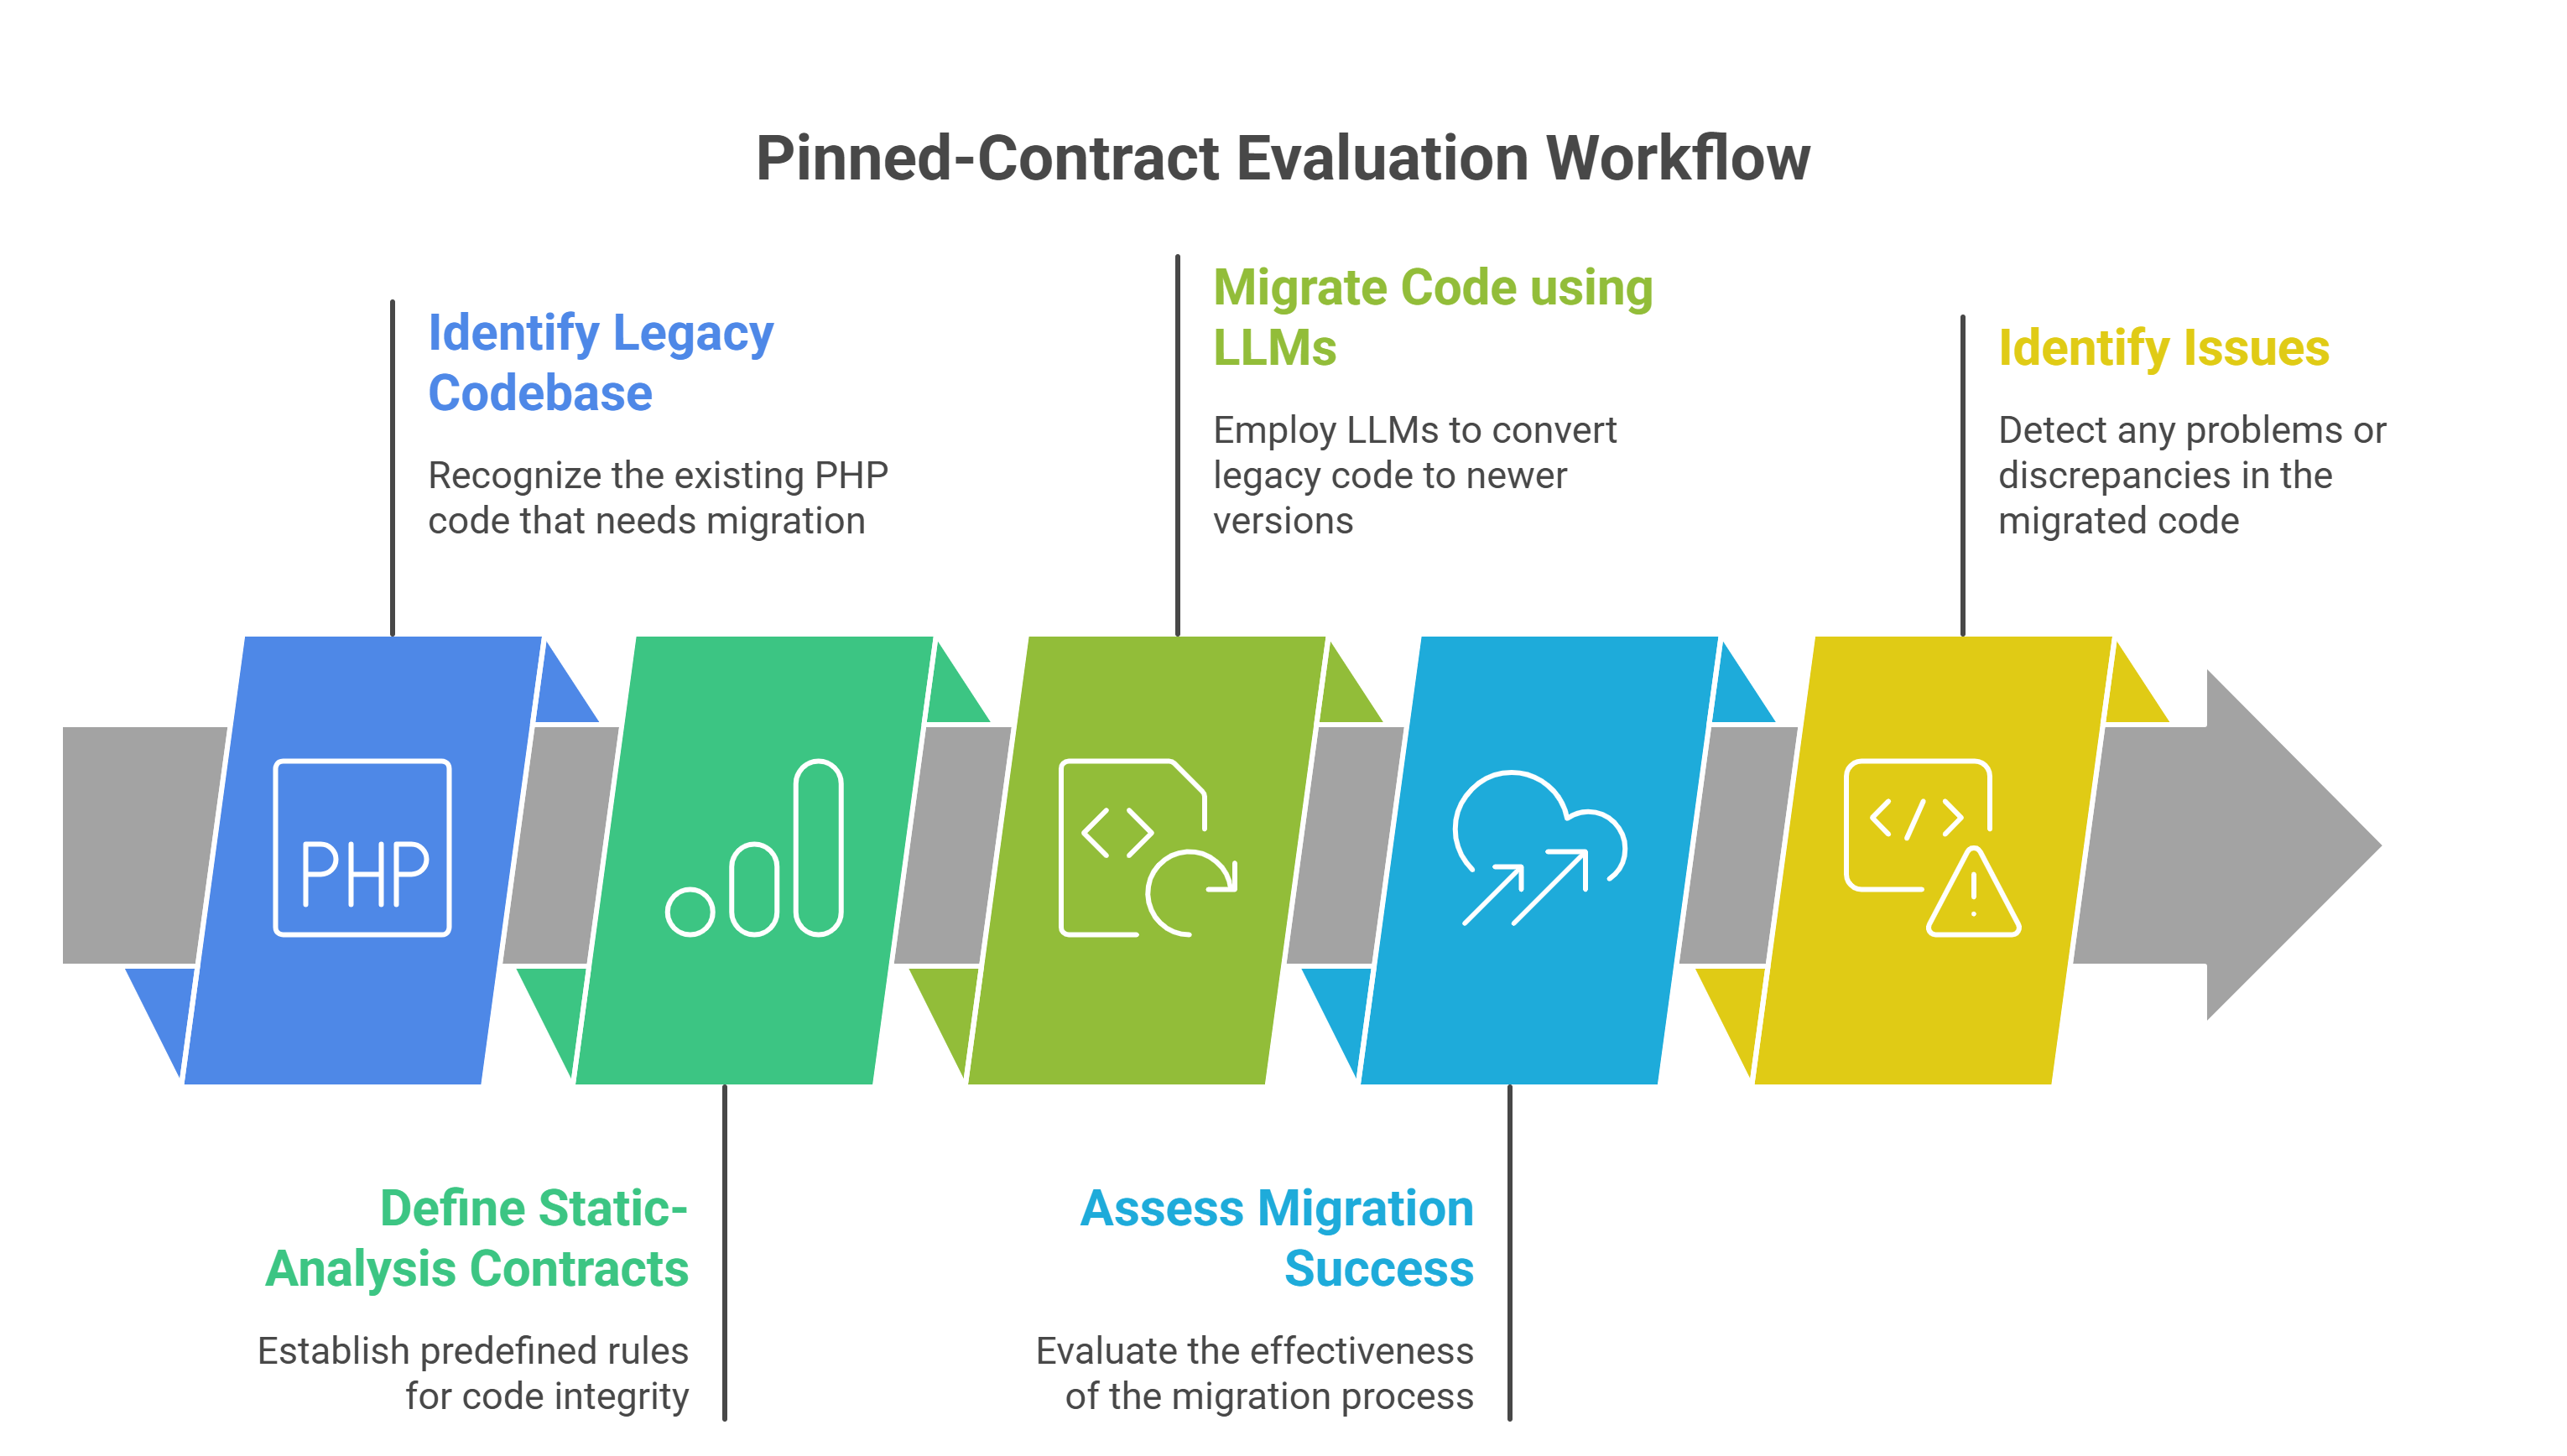
\includegraphics[width=\textwidth]{images/PCE-Pipeline.png}
\caption{Pinned-Contract Evaluation workflow. The process begins by identifying legacy PHP code, defining static-analysis contracts, migrating code using LLMs, assessing migration success, and detecting remaining issues.}
\label{fig:pce-workflow}
\end{figure*}

\section{Introduction}
\label{sec:introduction}

PHP continues to power a large portion of production web software, much of it in long-lived legacy systems.\cite{w3techs_php,w3techs_wordpress,wordpress}
Migrating these systems to newer PHP versions is difficult.
Required changes are scattered across the codebase and span evolving language features, library updates, and stricter typing constraints.\cite{php83spec,persson2015php}
Developers need visibility not only into whether a migration succeeds, but also into which upgrade requirements are satisfied and which remain unresolved.

Large language models are increasingly used to assist software modernization, yet evaluating their effectiveness remains challenging.
Most existing studies rely on outcome signals such as parsing success, linting results, or test outcomes.\cite{openai2023gpt4,roziere2023codellama,cassano2024canitedit}
These signals are useful, but they provide limited insight into what changed during migration.
They show whether code runs, but they do not reveal which upgrade obligations were resolved or newly introduced.
This limits systematic comparison across models and prompting strategies, especially when performance varies with context limits and input size.\cite{liu2024lost,du2025context,jimenez2024swebench}

We introduce \textbf{Pinned Contract Evaluation (PCE)}, a policy-grounded framework for evaluating automated code modernization.
PCE treats a static analysis upgrade pipeline as a versioned migration contract.
Executing the contract on the original program induces an obligation space defined by triggered upgrade rule types.
Running the same contract on migrated outputs reveals which obligations are discharged, which remain, and which new ones appear.
Because the policy is fixed, results are directly comparable across systems and experiments.
PCE evaluates progress relative to a fixed upgrade policy rather than attempting to establish full behavioral or semantic correctness.
Unlike prior evaluations that treat static-analysis outputs only as coarse outcome signals, PCE formalizes the upgrade policy itself as a contract that induces a measurable obligation space for systematic comparison across systems.

To contextualize contract-level progress, we include additional diagnostics.
These include syntax validation, structural preservation signals, compatibility analysis using PHPCompatibility, and a regression-oriented loadability sentinel.

We instantiate PCE for PHP version migration using a pinned Rector upgrade pipeline.\cite{rector}
Across five LLM systems evaluated on a 100-file WordPress 4.0 benchmark, mean obligation discharge ranges from 38\% to 78\%.
Remaining work concentrates in PHP 8 rule families, and high discharge does not necessarily imply syntactic or runtime robustness.
These findings show why policy-grounded evaluation is useful for understanding both progress and failure modes in automated modernization.

\paragraph{Contributions}
This paper makes three contributions.

\begin{enumerate}[leftmargin=*]

\item \textbf{Pinned Contract Evaluation (PCE).}
A reproducible evaluation framework that models modernization as progress through a contract-induced obligation space defined by a pinned static analysis policy.

\item \textbf{Contract-induced migration benchmark.}
A 100-file WordPress 4.0 dataset that preserves the obligation space induced by the contract.

\item \textbf{Reproducible evaluation harness.}
A standardized LLM migration and scoring pipeline with deterministic extraction, reconstruction, and fully logged artifacts.

\end{enumerate}

\subsection{Research Questions}
\label{sec:rqs}

Under a fixed contract and its induced obligation space, we ask:

\begin{enumerate}[leftmargin=*]

\item RQ1. How do models compare in obligation discharge and residual obligation profiles?

\item RQ2. Which rules and language milestones remain most resistant to automated migration?

\item RQ3. How does contract progress relate to syntax validity, structural preservation, and loadability regressions?

\item RQ4. How do PCE outcomes align with results from an independent compatibility analysis using PHPCompatibility?

\end{enumerate}

\subsection{Artifacts and Code Availability}
\label{subsec:artifacts}

We release all prompts, configurations, benchmark metadata, and evaluation scripts in a public repository to enable independent reproduction of our results.\cite{wohlin2012experimentation}
\section{Related Work}
\label{sec:related}

Empirical studies of migration tools often report end-state signals such as compilation success, linting results, test outcomes, or manual inspection. These signals provide coarse evidence of success but rarely attribute progress to specific upgrade requirements. They also make cross-study comparison difficult when toolchains and configurations differ. In this work we instead evaluate modernization against an explicit and fixed upgrade policy.

\paragraph*{Rule-based migration}
Refactoring and API evolution are well studied.\cite{DBLP:journals/tse/MensT04,DBLP:conf/oopsla/DigJ06,fowler1999refactoring,henkel2005catchup}
Rule-based tools encode curated transformations.\cite{DBLP:conf/icse/Murphy-HillPB09,rector}
They scale because rewrites are deterministic.\cite{openrewrite,errorprone,refaster,facebook_codemod}
However, many migrations require non-local reasoning. Dependencies, type flow, and framework conventions limit rule coverage.\cite{DBLP:conf/icse/Murphy-HillPB09,mccabe1976complexity,chidamber1994metrics}
Residual work therefore remains common in large systems.\cite{wittern2016api}
Semantic patching increases expressiveness but remains fundamentally rule driven.\cite{coccinelle}

\paragraph*{LLM-assisted refactoring and migration}
LLMs can generate edits beyond predefined rules.\cite{chen2021codex,nijkamp2022codegen,li2022alphacode,ouyang2022instructgpt,touvron2023llama}
Benchmarks evaluate editing, translation, and issue resolution.\cite{cassano2024canitedit,jimenez2024swebench,swebench_verified}
Long-context limits complicate their application to large codebases.\cite{liu2024lost,du2025context}
Despite this progress, evaluations of LLM-based migration still rely primarily on coarse outcome signals such as parsing, linting, or tests.\cite{openai2023gpt4,roziere2023codellama}
These signals indicate whether code runs but do not reveal which upgrade requirements were satisfied or how migration progress distributes across rule types.

\paragraph*{Static analysis and compatibility checking}
Static analysis is widely used in maintenance and automated repair and can scale to large codebases.\cite{legoues2012genprog,DBLP:conf/icse/NguyenQRC13,DBLP:conf/issta/MartinezM16,DBLP:conf/issta/JustJE14,DBLP:conf/icse/GazzolaMM18,bessey2010billion,calcagno2015moving}
In the PHP ecosystem, tools such as Rector and PHPCompatibility map findings to version targets.\cite{phpcompat,rector,php83spec}
However, results depend heavily on tool versions and configuration choices, which complicates cross-study comparison.
Other work measures change using fine-grained differencing or test coverage.\cite{fluri2007change,falleri2014fine,kochhar2015coverage}
While useful, these approaches still treat static-analysis outputs as signals rather than as a formal evaluation policy.

\paragraph*{Positioning of this work}
We introduce \emph{Pinned Contract Evaluation (PCE)}.
Our key idea is to treat a pinned static-analysis configuration as an explicit migration contract.
Executing this contract on the original code induces an obligation space defined by triggered upgrade rules.
Running the same contract on migrated outputs reveals which obligations were discharged and which new ones were introduced.
By fixing the analysis policy, PCE enables controlled, reproducible, and fine-grained comparison of automated modernization systems—something prior evaluation approaches do not explicitly provide.
\section{Pinned Contract Benchmark Construction}
\label{sec:benchmark_construction}

We construct a 100-file benchmark from WordPress~4.0 to evaluate migration under a pinned Rector contract.
The contract is a fixed Rector version, ruleset, and configuration.
We chose WordPress because it is large, long-lived, and exhibits substantial PHP version drift.

The benchmark is diagnostic by design.
We do not try to match the natural WordPress file distribution.
Instead, we optimize for coverage of the contract-induced obligation space.
Here, the obligation space is the set of Rector upgrade rule types that trigger in the corpus.
This choice makes results easier to interpret.
It also prevents rare but important obligations from being obscured by project-specific frequency effects.
The benchmark therefore measures progress against the pinned policy, not typicality of WordPress workloads.
This design preserves the full contract-induced rule space, enabling controlled and reproducible comparison of automated migration systems under a fixed upgrade policy.

The design follows standard guidance for controlled empirical studies and reproducible benchmark construction.\cite{wohlin2012experimentation}

\paragraph{Overview}
We build the benchmark in three steps:
\begin{enumerate}[leftmargin=*]
\item Run the pinned contract on the full corpus to obtain baseline triggers.
\item Characterize the triggered rule space (Table~\ref{tab:coverage_dimensions}).
\item Select 100 files using size stratification while preserving all rule types (Appendix~\ref{app:benchmark_algorithms}).
\end{enumerate}

We also define a 55-file execution slice.
We use it only as a loadability sentinel.
It flags new include-time failures under a fixed harness.
We interpret it only as a regression signal.

\begin{table}[htbp]
\centering
\caption{Coverage analysis dimensions used to characterize the triggered rule space under the pinned contract.}
\label{tab:coverage_dimensions}
\small
\begin{tabular}{@{}l p{0.50\columnwidth}@{}}
\toprule
\textbf{Dimension} & \textbf{Description} \\
\midrule
Rule type frequency & Corpus frequency of each Rector upgrade rule type. \\
PHP version mapping & Mapping rules to PHP~5.x, 7.x, and 8.x milestone families. \\
Rule categories & Distribution across AST constructs such as \texttt{FuncCall}, \texttt{Array\_}, and \texttt{Class\_}. \\
Size and complexity & Relationship between LOC and rule diversity. \\
Tail coverage & Preservation of infrequent rule types during sampling. \\
\bottomrule
\end{tabular}
\end{table}

\subsection{Inducing Contract Findings}
\label{sec:benchmark_static_analysis}

We analyze the full WordPress~4.0 corpus (482 PHP files) with the reference Rector configuration.
We pin \texttt{LevelSetList::UP\_TO\_PHP\_83} and the tool versions.
This keeps the contract stable across runs.
Static analysis triggers provide a consistent signal at scale.\cite{bessey2010billion,calcagno2015moving}

We record findings as file-level rule incidence.
A rule counts once per file if it triggers.
We use incidence because it is stable across repeated runs and configurations.
In-file counts are not consistently exposed by Rector.

We also record Rector dry-run patches.
They summarize edits suggested by the pinned contract.
We use them as a proxy for residual patch volume.\cite{falleri2014fine,fluri2007change}

Across the corpus we observe 1{,}331 file rule incidences spanning 48 upgrade rules.
This defines the obligation space used for benchmark construction and scoring.

\begin{table}[htbp]
\centering
\caption{Scoring criteria for size-stratified file selection.}
\label{tab:selection_criteria}
\small
\begin{tabular}{@{}l p{0.50\columnwidth}@{}}
\toprule
\textbf{Criterion} & \textbf{Role in File Selection} \\
\midrule
Rule diversity & Prefer files triggering many rule types. \\
Version change density & Reward stronger evidence of version-related changes. \\
Size suitability & Favor 100 to 2000 LOC and penalize very large files. \\
PHP family breadth & Prefer files spanning multiple rule families. \\
Key patterns & Extra weight for migration-relevant constructs. \\
\bottomrule
\end{tabular}
\end{table}

\subsection{Coverage Preserving Selection}
\label{sec:benchmark_selection}

We summarize baseline triggers to measure rule frequency, milestone coverage, and size effects.
Rare rule types matter, but uniform sampling can drop them.
We therefore enforce full rule coverage during selection.

Selection has two steps.
First, we stratify files by size and rank them using Table~\ref{tab:selection_criteria}.
Second, we enforce full rule coverage and trim to exactly 100 files while preserving coverage.
The procedure is deterministic.
We fix it before running any LLM experiments.

\begin{table}[htbp]
\centering
\caption{Target size distribution used for stratified initialization. The realized benchmark may differ after coverage enforcement.}
\label{tab:size_distribution}
\small
\begin{tabular}{@{}l c c@{}}
\toprule
\textbf{Category} & \textbf{LOC Range} & \textbf{Share} \\
\midrule
Small & 1--200 & 35\% \\
Medium & 201--500 & 30\% \\
Large & 501--1000 & 25\% \\
Extra large & 1001+ & 10\% \\
\bottomrule
\end{tabular}
\end{table}

\begin{table}[htbp]
\centering
\caption{Average migration complexity by file size in the released benchmark.}
\label{tab:migration_complexity}
\small
\begin{tabular}{@{}l c c c@{}}
\toprule
\textbf{Category} & \textbf{Files} & \textbf{Trig./File} & \textbf{Ver./File} \\
\midrule
Small & 31 & 3.2 & 2.9 \\
Medium & 31 & 5.4 & 4.8 \\
Large & 26 & 5.7 & 5.0 \\
Extra large & 12 & 8.9 & 6.2 \\
\bottomrule
\end{tabular}
\end{table}

\subsection{Benchmark Integrity}
\label{sec:benchmark_validation}

All selected files run through the pinned contract successfully.
The benchmark preserves all 48 upgrade rules.
It induces 521 file rule incidences spanning PHP~5.2 to 8.3.
Larger files trigger more rule types and span more milestones (Table~\ref{tab:migration_complexity}).
This matches prior links between structural complexity and transformation diversity.\cite{chidamber1994metrics,mccabe1976complexity}

Because coverage is the hard constraint, the final size mix can differ slightly from Table~\ref{tab:size_distribution}.

We also define a 55-file loadability slice.
We report only new failures (original pass, migrated fail) under the same harness.
We do not treat absolute pass rates as behavioral correctness.
\section{LLM-Based PHP Version Migration Framework}
\label{sec:migration_framework}

We implement a controlled framework for LLM-assisted PHP migration.
It standardizes prompting, context handling, and reconstruction.
The goal is to reduce orchestration variance.
Differences should reflect model behavior, not pipeline artifacts.
Rector is used only for evaluation as the pinned contract.\cite{rector}
The migration procedure is model- and provider-agnostic.

\paragraph{Design principles}
We enforce three constraints.
First, systems share the same degrees of freedom.
We fix prompts, chunking policy, and decoding settings where supported.
Second, extraction and reconstruction are deterministic from recorded responses.
Third, we surface failures.
Timeouts and extraction failures are reported, not repaired.
This isolates model behavior and supports fair comparison.

\subsection{Configuration and provider interface}
\label{sec:framework_config}

A centralized configuration defines model identifiers, request limits, and decoding settings where supported.
We log prompts, responses, and run metadata for audit and recomputation.

A unified provider interface normalizes authentication, request formatting, and error handling.
This keeps the migration policy consistent across systems.

\subsection{Migration policy and context management}
\label{sec:framework_chunking}

We treat context length as a fixed constraint.\cite{liu2024lost,du2025context}
Files up to 500 lines use one request.
Longer files are split to fit a bounded budget.
We use line count as a provider-agnostic proxy for request size.
Chunk boundaries depend only on the input file and pinned parameters.

We use a fixed PHP-aware boundary heuristic to reduce mid-function splits (Appendix~\ref{app:benchmark_algorithms}).
We do not use learned or adaptive chunking.

We disable overlap, retrieval augmentation, multi-pass refinement, and cross-chunk repair.
Each model runs a single-pass policy under the same constraints.

Prompts require begin and end markers.
Whole-file outputs are used directly.
Chunk outputs are concatenated in order.

\subsection{Output extraction and reconstruction}
\label{sec:framework_reconstruction}

Responses must place migrated code between markers.
The parser checks marker presence and extracts only the enclosed code.
For chunked files, we reconstruct outputs by ordered concatenation.

If extraction fails for a chunk, we insert a fixed placeholder comment that reports the failure.
We do not attempt heuristic repair.
Failures propagate to syntax checks and contract scoring.
This prevents inflated results.

We store all artifacts with raw responses and execution metadata.
This supports inspection and reproducibility.

\subsection{Experimental orchestration}
\label{sec:framework_orchestration}

The orchestration layer applies the fixed policy, records extraction outcomes, and prepares outputs for contract evaluation.
This yields consistent experimental conditions and fully traceable runs.



\section{Pinned Contract Evaluation}
\label{sec:rector_eval}



\subsection{Objective and pinned instrument}
\label{sec:pce_objective_instrument}

PCE measures modernization as \emph{progress against a fixed upgrade policy}, rather than as full functional correctness.
We encode the policy as a \emph{pinned} Rector configuration with a fixed Rector version, ruleset, and parameters.\cite{rector}
We treat this configuration as a migration contract.

We apply the contract twice.
First, we run it on the original benchmark.
For each file, the contract emits a set of upgrade \emph{rule types} that trigger, and this set defines that file's \emph{obligations} under the policy.
Second, we run the same contract on migrated outputs and measure (i) which baseline obligations no longer trigger (discharged obligations) and (ii) which new rule types now trigger (introduced obligations, meaning contract-visible regressions).
If Rector cannot analyze a migrated file (e.g., parser/runtime failure during dry-run), we exclude that file from PCE aggregates for that model and report analyzed coverage.

To focus on language migration, we score only \texttt{Rector\textbackslash Php*} rules.
We report additional diagnostics to contextualize contract outcomes (Section~\ref{sec:pce_validity_diagnostics}) and triangulate with PHPCompatibility (Section~\ref{sec:pce_phpcompat}).\cite{phpcompat}

\subsection{Signals: compliance breadth and residual-work proxy}
\label{sec:pce_primary_scores}

PCE reports two complementary signals.

\textbf{(1) Obligation discharge (primary).}
This measures breadth of compliance, meaning how much of the contract-defined obligation set is cleared.
Our unit of analysis is a \emph{file-level rule-type incidence}: a rule type counts at most once per file, regardless of how many times it occurs within that file.

\textbf{(2) Patch volume closure (secondary).}
This summarizes how much Rector dry-run patch volume remains after migration.
We use it only as a diff-magnitude proxy, not as developer effort.

% =========================
% Per-file metrics table
% (ICSE-style: compact, declarative, minimal prose)
% =========================
\begin{table}[t]
\centering
\caption{Per-file metrics recorded under the pinned contract.}
\label{tab:per_file_eval_metrics}
\small
\setlength{\tabcolsep}{4pt}
\renewcommand{\arraystretch}{1.12}
\begin{tabularx}{\columnwidth}{@{}>{\raggedright\arraybackslash}p{0.34\columnwidth} >{\raggedright\arraybackslash}X@{}}
\toprule
\textbf{Metric} & \textbf{Definition / description} \\
\midrule
Original triggers ($\mathcal{O}_i$, $O_i$) &
Rule \emph{types} triggered in file $i$ pre-migration; $O_i=|\mathcal{O}_i|$. \\
Remaining triggers ($\mathcal{R}_i$, $R_i$) &
Rule \emph{types} triggered post-migration; $R_i=|\mathcal{R}_i|$. \\
Removed / introduced ($S_i$, $I_i$) &
$S_i=|\mathcal{O}_i\setminus\mathcal{R}_i|$;\;
$I_i=|\mathcal{R}_i\setminus\mathcal{O}_i|$. \\
Net change ($\Delta_i$) &
$\Delta_i=S_i-I_i$ (negative: more types introduced). \\
Discharge rate ($\rho_i$) &
$\rho_i=\frac{S_i}{O_i}\times 100$. \\
Patch volume ($D_i$) &
Changed-line count in Rector dry-run patch (\texttt{diff\_line\_count}); residual edit-mass proxy. \\
Patch closure (\%) &
Closure relative to $D_i^{\mathrm{orig}}$ (WDC, MFDC). \\
Metadata &
LOC, size bin, identifiers; residual set $\mathcal{R}_i$ and milestone/rule breakdowns. \\
\bottomrule
\end{tabularx}
\end{table}
% =========================
% Outcome matrices table (syntax + loadability)
% =========================
\begin{table}[t]
\centering
\caption[Outcome matrices for syntax and loadability]{Outcome matrices for syntax lint and the isolated \emph{loadability tripwire} (regression-oriented: Orig.\ Pass $\rightarrow$ Migr.\ Fail).}
\label{tab:outcome_matrices}
\scriptsize
\setlength{\tabcolsep}{3pt}
\renewcommand{\arraystretch}{1.05}
\begin{subtable}[t]{0.46\columnwidth}
\centering
\caption{Syntax}
\label{tab:syntax_validation_outcomes}
\begin{tabular}{@{}lcc@{}}
\toprule
Outcome & Orig. & Migr. \\
\midrule
Both valid  & Pass & Pass \\
Fixed error & Fail & Pass \\
New error   & Pass & Fail \\
Both error  & Fail & Fail \\
\bottomrule
\end{tabular}
\end{subtable}
\hspace{6pt}
\begin{subtable}[t]{0.46\columnwidth}
\centering
\caption{Loadability}
\label{tab:runtime_validation_outcomes}
\begin{tabular}{@{}lcc@{}}
\toprule
Outcome & Orig. & Migr. \\
\midrule
Both pass     & Pass & Pass \\
Fixed failure & Fail & Pass \\
New failure   & Pass & Fail \\
Both fail     & Fail & Fail \\
\bottomrule
\end{tabular}
\end{subtable}
\end{table}

% =========================
% Structural diagnostics table
% =========================
\begin{table}[t]
\centering
\caption{Structural preservation signals.}
\label{tab:structural_completeness_signals}
\small
\setlength{\tabcolsep}{4pt}
\renewcommand{\arraystretch}{1.10}
\begin{tabularx}{\columnwidth}{@{}l X@{}}
\toprule
\textbf{Signal} & \textbf{Purpose} \\
\midrule
Token dist.\ sim. & Token-type frequency similarity (non-trivia). \\
Token seq.\ sim.  & Order-sensitive similarity on normalized token stream. \\
Decl.\ overlap    & Set overlap of namespaces/classes/functions/methods. \\
Line preservation & Code-line retention (excluding blank/comment lines). \\
Body preservation & Body token retention for matched declarations. \\
Signature stability & Parameter/modifier consistency for matched declarations. \\
Empty-body rate   & Fraction of matched bodies that are near-empty. \\
Trivial-stub rate & Fraction of matched bodies with shallow stub patterns. \\
\midrule
\multicolumn{2}{@{}p{\columnwidth}@{}}{\footnotesize\emph{Note:} Body/stub signals apply only when bodies exist; otherwise N/A.} \\
\bottomrule
\end{tabularx}
\end{table}

\subsubsection{Breadth: obligation discharge}
\label{sec:pce_breadth}

For file $i$, let $\mathcal{O}_i$ be the set of rule types that trigger on the original file under the pinned contract, and let $\mathcal{R}_i$ be the set that trigger on the migrated output.
Let $O_i = |\mathcal{O}_i|$ and $R_i = |\mathcal{R}_i|$.

We decompose change into three quantities:
\[
\begin{aligned}
S_i &= |\mathcal{O}_i \setminus \mathcal{R}_i|
\quad \text{(discharged types)}, \\
I_i &= |\mathcal{R}_i \setminus \mathcal{O}_i|
\quad \text{(introduced types)}, \\
\Delta_i &= S_i - I_i
\quad \text{(net change)}.
\end{aligned}
\]
Intuitively, $S_i$ answers: ``How many baseline rule types stopped triggering in this file?''
$I_i$ answers: ``How many new rule types did the migration introduce under the same policy?''

We define the per-file discharge rate as:
\[
\rho_i = \frac{S_i}{O_i}\times 100.
\]
All benchmark files satisfy $O_i>0$ by construction.
We report $I_i$ explicitly to surface contract-visible regressions.
These are not behavioral claims, only new triggers under the pinned policy.

\subsubsection{Secondary proxy: patch volume closure}
\label{sec:pce_depth}

Let $D_i$ be Rector's dry-run changed-line count for file $i$ on the migrated output, and let $D_i^{\mathrm{orig}}$ be the same quantity on the original file under the same pinned contract.
We summarize reduction in patch volume in two ways: (i) workload-weighted closure (WDC), which emphasizes high-volume files, and (ii) mean file-level closure (MFDC), which treats files uniformly.
If either quantity is missing or unreadable for a file (e.g., failed Rector analysis output), that file is excluded from numeric patch-volume aggregates.

\providecommand{\WDC}{\textnormal{WDC}}
\providecommand{\MFDC}{\mathrm{MFDC}}
{\footnotesize
\begin{align}
\WDC(m)
&= \left(1-\frac{\sum_i D_i^{m}}{\sum_i D_i^{\mathrm{orig}}}\right)\cdot 100,\\
\MFDC(m)
&= \frac{1}{N}\sum_i c_i,\\[-2pt]
c_i
&=
\begin{aligned}[t]
\left(1-\frac{D_i^{m}}{D_i^{\mathrm{orig}}}\right)\cdot 100 \;& (D_i^{\mathrm{orig}}>0)\\
100 \;& (D_i^{\mathrm{orig}}=0,\, D_i^{m}=0)\\
0 \;& (D_i^{\mathrm{orig}}=0,\, D_i^{m}>0)\;.
\end{aligned}
\end{align}
}
Patch volume closure can be inflated by stylistic rewrites or diff-shaping changes, so we use it only as supporting context for residual work, not as a correctness or effort estimate.



\subsection{Reporting and interpretation}
\label{sec:pce_interpretation}

For each file we record the obligation counts and changes ($O_i, R_i, S_i, I_i, \Delta_i, \rho_i$) and patch volume ($D_i$), together with metadata and diagnostics (Table~\ref{tab:per_file_eval_metrics}).

At the model level we report mean and median discharge, and a workload-weighted discharge:
\[
\rho_w =
\frac{\sum_{i=1}^{N} S_i}{\sum_{i=1}^{N} O_i}\times 100,
\]
which answers: ``Across all baseline obligations, what fraction were discharged?''
We summarize patch closure using WDC and MFDC, and report concentration statistics (median, P95, top-five share) to expose heavy-tailed residual work.

We interpret $I_i$ and $\Delta_i$ only as contract regressions, meaning new triggers under the pinned policy.
They are not behavioral regressions.
Contract metrics are therefore read together with validity, preservation, and loadability diagnostics.

\subsection{Validity and regression diagnostics}
\label{sec:pce_validity_diagnostics}

Contract metrics can be misleading in the presence of omissions, degenerate rewrites, syntax errors, or include-time failures.
Accordingly, we report a fixed diagnostic suite for every output to contextualize contract outcomes.
These checks provide signals of validity and regressions, but they do not establish functional equivalence.

\paragraph{Diagnostic tiers}
We report:
(i) syntax validation via \texttt{php -l} (PHP~8.3),
(ii) structural preservation signals (Table~\ref{tab:structural_completeness_signals}),
(iii) contract metrics under Rector,
(iv) PHPCompatibility results, and
(v) a loadability sentinel (Section~\ref{sec:pce_loadability}).
Outcome definitions appear in Table~\ref{tab:outcome_matrices}.
Metrics that require parsing are N/A when \texttt{php -l} fails.

\subsection{Isolated loadability sentinel}
\label{sec:pce_loadability}

We run a loadability sentinel on a fixed slice ($N_{\mathrm{rt}}=55$).
Each file is loaded once via \texttt{require\_once} in a minimal WordPress stub harness.
Parse errors, fatal errors, and uncaught exceptions count as failures.
We interpret this tier only as a regression signal.
A regression is orig pass and migrated fail.

% =========================
% Results table 
% =========================
\begin{table*}[t]
\centering
\caption[Evaluation summary under pinned contract]{Pinned-contract evaluation on the coverage-optimized diagnostic stress test. All quantities are contract-relative. Panel A reports the primary outcome (incidence-level discharge). Panel B stratifies discharge by file size. Panel C reports discharge by PHP family. Patch-volume closure is reported for localization only (not effort).}
\label{tab:results_panels_revised}
\footnotesize
\setlength{\tabcolsep}{4pt}
\renewcommand{\arraystretch}{1.12}

% ---------------- Panel A ----------------
\textbf{A. Obligation discharge (incidence-level breadth; pinned contract)}\par
\vspace{2pt}
\resizebox{\textwidth}{!}{%
\begin{tabular}{lrrrrrrrr}
\toprule
\textbf{System} &
\textbf{Mean $\rho$ (\%)} &
\textbf{Weighted $\rho_w$ (\%)} &
\textbf{Discharged} &
\textbf{Remaining} &
\textbf{Introduced} &
\textbf{Net $\Delta$} &
\textbf{complete} &
\textbf{$\rho_i<50\%$} \\
\midrule
Rector-applied (reference)   & 98.55 & 98.43 & 503 & 17  & 9 & 494 & 89 & 0  \\
\midrule
Gemini 2.5 Pro               & 77.11 & 75.76 & 372 & 140 & 21 & 351 & 19 & 3  \\
Gemini 2.5 Flash             & 62.32 & 59.48 & 273 & 203 & 17 & 256 & 13 & 24 \\
GPT-5 Codex                  & 71.35 & 69.39 & 297 & 151 & 20 & 277 & 15 & 12 \\
Claude Sonnet 4 (2025-05-14) & 56.97 & 54.51 & 272 & 244 & 17 & 255 & 6  & 33 \\
Llama 3.3 70B Instruct       & 34.21 & 32.16 & 156 & 347 & 18 & 138 & 2  & 66 \\
\bottomrule
\end{tabular}%
}
\vspace{2pt}
\noindent\footnotesize Aggregates are computed over analyzable files per model after excluding migrated files where Rector dry-run failed: Rector 100, Claude 97, Gemini Flash 91, Gemini Pro 97, GPT-5 Codex 88, Llama 95.\normalsize

% ---------------- Panel B ----------------
\textbf{B. Obligation discharge by file size (Mean $\rho$; discharged/total incidences)}\par
\vspace{2pt}
{\scriptsize
\resizebox{\textwidth}{!}{%
\begin{tabular}{lcccc}
\toprule
\textbf{Model} &
\textbf{Small} &
\textbf{Medium} &
\textbf{Large} &
\textbf{Extra-large} \\
\midrule
Gemini 2.5 Pro &
77.63 (77/99) & 83.81 (136/162) & 74.76 (105/141) & 60.58 (54/89) \\
Gemini 2.5 Flash &
71.51 (70/99) & 66.97 (104/153) & 51.22 (67/131)  & 41.84 (32/76) \\
GPT-5 Codex &
75.86 (76/99) & 75.88 (111/146) & 66.58 (86/130) & 45.13 (24/53) \\
Claude Sonnet 4 (2025-05-14) &
65.75 (60/91) & 69.33 (111/158) & 41.53 (63/146)  & 38.30 (38/104) \\
Llama 3.3 70B Instruct &
37.76 (35/93) & 42.70 (71/162) & 28.50 (40/140) & 11.85 (10/90) \\
\bottomrule
\end{tabular}%
}}
\vspace{2pt}

% ---------------- Panel C ----------------
\noindent\textbf{C. Discharged obligations by PHP family (analyzable subset per model; discharged/total; \% discharged)}\par
\vspace{2pt}
\begin{tabular*}{\textwidth}{@{\extracolsep{\fill}}p{0.30\textwidth}ccc@{}}
\toprule
\textbf{Model} & \textbf{PHP 5.x} & \textbf{PHP 7.x} & \textbf{PHP 8.x} \\
\midrule
Gemini 2.5 Flash & 116/137 (84.67\%) & 97/120 (80.83\%) & 60/202 (29.70\%) \\
Gemini 2.5 Pro   & 143/149 (95.97\%) & 114/126 (90.48\%) & 115/216 (53.24\%) \\
GPT-5 Codex      & 126/133 (94.74\%) & 88/106 (83.02\%) & 83/189 (43.92\%) \\
Claude Sonnet 4 (2025-05-14) & 109/150 (72.67\%) & 92/129 (71.32\%) & 71/220 (32.27\%) \\
Llama 3.3 70B Instruct & 87/145 (60.00\%) & 53/125 (42.40\%) & 16/215 (7.44\%) \\
\bottomrule
\end{tabular*}
\vspace{4pt}

% --------- Supplementary ----------
\noindent\hrule height 0.4pt
\vspace{4pt}
\noindent\textbf{Secondary: Patch-volume closure (pinned contract; localization only)}\par
\vspace{2pt}
\begin{tabular*}{\textwidth}{@{\extracolsep{\fill}}p{0.30\textwidth}rrrr@{}}
\toprule
\textbf{System} &
\textbf{WDC (\%)} &
\textbf{MFDC (\%)} &
\textbf{Top-5 share (\%)} &
\textbf{Remaining patch lines} \\
\midrule
Rector-applied (reference)   & 95.08 & 98.19 & 91.43 & 1{,}109  \\
GPT-5 Codex                  & 67.46 & 69.93 & 36.46 & 5{,}074  \\
Gemini 2.5 Pro               & 71.92 & 76.90 & 50.70 & 5{,}826  \\
Gemini 2.5 Flash             & 60.65 & 64.75 & 43.53 & 7{,}620  \\
Claude Sonnet 4 (2025-05-14) & 57.77 & 62.75 & 40.31 & 9{,}411  \\
Llama 3.3 70B Instruct       & 36.71 & 42.33 & 39.35 & 12{,}342 \\
\bottomrule
\end{tabular*}
\end{table*}

\subsection{Cross-instrument triangulation with PHPCompatibility}
\label{sec:pce_phpcompat}

We triangulate using PHPCompatibility.\cite{phpcompat}
For each output set we run PHPCS with \texttt{--standard=PHPCompatibility} and \texttt{--runtime-set testVersion 8.3}.
We parse JSON reports and compute issue reduction:
\[
\text{IssueReduction}(\%)=
\frac{\text{Issues}_{\mathrm{orig}}-\text{Issues}_{\mathrm{model}}}
{\text{Issues}_{\mathrm{orig}}}\times 100.
\]
PHPCompatibility uses a different rule set and granularity than Rector.
Agreement suggests consistent movement under both policies.
Divergence reflects policy differences rather than a contradiction.

\subsection{Pipeline completeness and residual concentration}
\label{sec:pce_completeness_concentration}

We report:
\begin{align}
N_{\mathrm{contract\text{-}clean}} &= |\{ i \mid R_i=0 \}|,\\
N_{\mathrm{low\text{-}compliance}} &= |\{ i \mid \rho_i<50 \}|.
\end{align}
$N_{\mathrm{contract\text{-}clean}}$ counts files with no remaining triggers and captures breadth only.
$N_{\mathrm{low\text{-}compliance}}$ counts files with discharge below $50\%$.
We also report concentration over remaining triggers and patch volume (median, P95, top-five share).

\subsection{Contract-aligned reference baseline}
\label{sec:pce_baseline}

We include a contract-aligned reference baseline, \emph{Rector applied}.
We apply the pinned ruleset to each file, then re-run the same contract on the rewritten output.

This baseline is not guaranteed to be trigger-free.
Rector rules are conservative and pattern-limited.
It provides a practical ceiling under the same policy and scoring protocol.

\section{Results}
\label{sec:results}

We evaluate five LLM systems under the pinned Rector contract
(Section~\ref{sec:rector_eval}), scoring only \texttt{Rector\textbackslash Php*}
rules. The primary outcome is all files weighted discharge,
$\rho_w^{\mathrm{all}}$. We interpret contract scores jointly with syntax,
preservation, loadability, and PHPCompatibility diagnostics.

\paragraph*{Overview}
Figure~\ref{fig:model_overview} highlights three properties of contract progress under the pinned policy.. First, PCE reveals
substantial variation in discharged upgrade work, with weighted discharge
from 30.53\% to 72.80\%
(Table~\ref{tab:contract_discharge_summary}). Second, residual work
concentrates in PHP~8.x families
(Table~\ref{tab:php_family_discharge}). Third, contract progress does not
subsume robustness: higher discharge can still coincide with syntax
failures, reduced preservation, and new loadability regressions
(Tables~\ref{tab:syntax_model_results},
\ref{tab:runtime_slice_results}). Agreement with PHPCompatibility is
therefore informative, but incomplete
(Table~\ref{tab:phpcompat_validation}).

% =================================================================
%  TABLE 1 — CONTRACT DISCHARGE SUMMARY
% =================================================================
\begin{table*}[t]
\centering
\caption{Obligation discharge under the pinned contract.
  Weighted $\rho_w^{\mathrm{all}}$ and Discharged use all-files scoring;
  remaining columns are computed on analyzable migrated files only.}
\label{tab:contract_discharge_summary}
\setlength{\tabcolsep}{4pt}
\renewcommand{\arraystretch}{1.18}
\resizebox{\textwidth}{!}{%
\begin{tabular}{%
  L{3.6cm}
  R{1.6cm}@{\hspace{4pt}}
  R{1.8cm}@{\hspace{4pt}}
  R{1.4cm}@{\hspace{4pt}}
  R{1.6cm}@{\hspace{4pt}}
  R{1.4cm}@{\hspace{4pt}}
  R{1.5cm}@{\hspace{4pt}}
  R{1.1cm}%
}
\arrayrulecolor{hdrBlue}
\toprule[1.5pt]
\tophdr{System} &
\tophdr{Mean $\rho$ (\%)} &
\tophdr{Wtd $\rho_w^{\mathrm{all}}$ (\%)} &
\tophdr{Dischgd} &
\tophdr{Post trig $R$} &
\tophdr{Introed} &
\tophdr{Ctr-clean} &
\tophdr{$\rho_i{<}50\%$} \\
\midrule[1pt]
% --- Reference -------------------------------------------------
\rowcolor{rowA}
\refrow{Rector (reference)} &
\refrow{98.55} & \refrow{98.43} & \refrow{503} &
\refrow{17}    & \refrow{9}    & \refrow{89}  & \refrow{0} \\
\midrule[0.4pt]
% --- LLMs ------------------------------------------------------
\rowcolor{rowB}
Gemini 2.5 Pro               & 77.11 & 72.80 & 372 & 140 & 21 & 19 & 3  \\
\rowcolor{rowA}
GPT-5 Codex                         & 71.35 & 58.12 & 297 & 151 & 20 & 15 & 12 \\
\rowcolor{rowB}
Gemini 2.5 Flash                    & 62.32 & 53.42 & 273 & 203 & 17 & 13 & 24 \\
\rowcolor{rowA}
Claude Sonnet 4 \scriptsize(05-14)  & 56.97 & 53.23 & 272 & 244 & 17 &  6 & 33 \\
\rowcolor{rowB}
Llama 3.3 70B Instruct      & 34.21 & 30.53 & 156 & 347 & 18 & 2 & 66 \\
\bottomrule[1.5pt]
\end{tabular}}
{\scriptsize\emph{Note.}
  Analyzable file counts: Rector 100, Claude 97, Gemini Flash 91,
  Gemini Pro 97, GPT-5 Codex 88, Llama 95.}
\end{table*}

% =================================================================
%  FIGURE — Model overview  (placed right after summary table)
% =================================================================
\begin{figure*}[t]
\centering
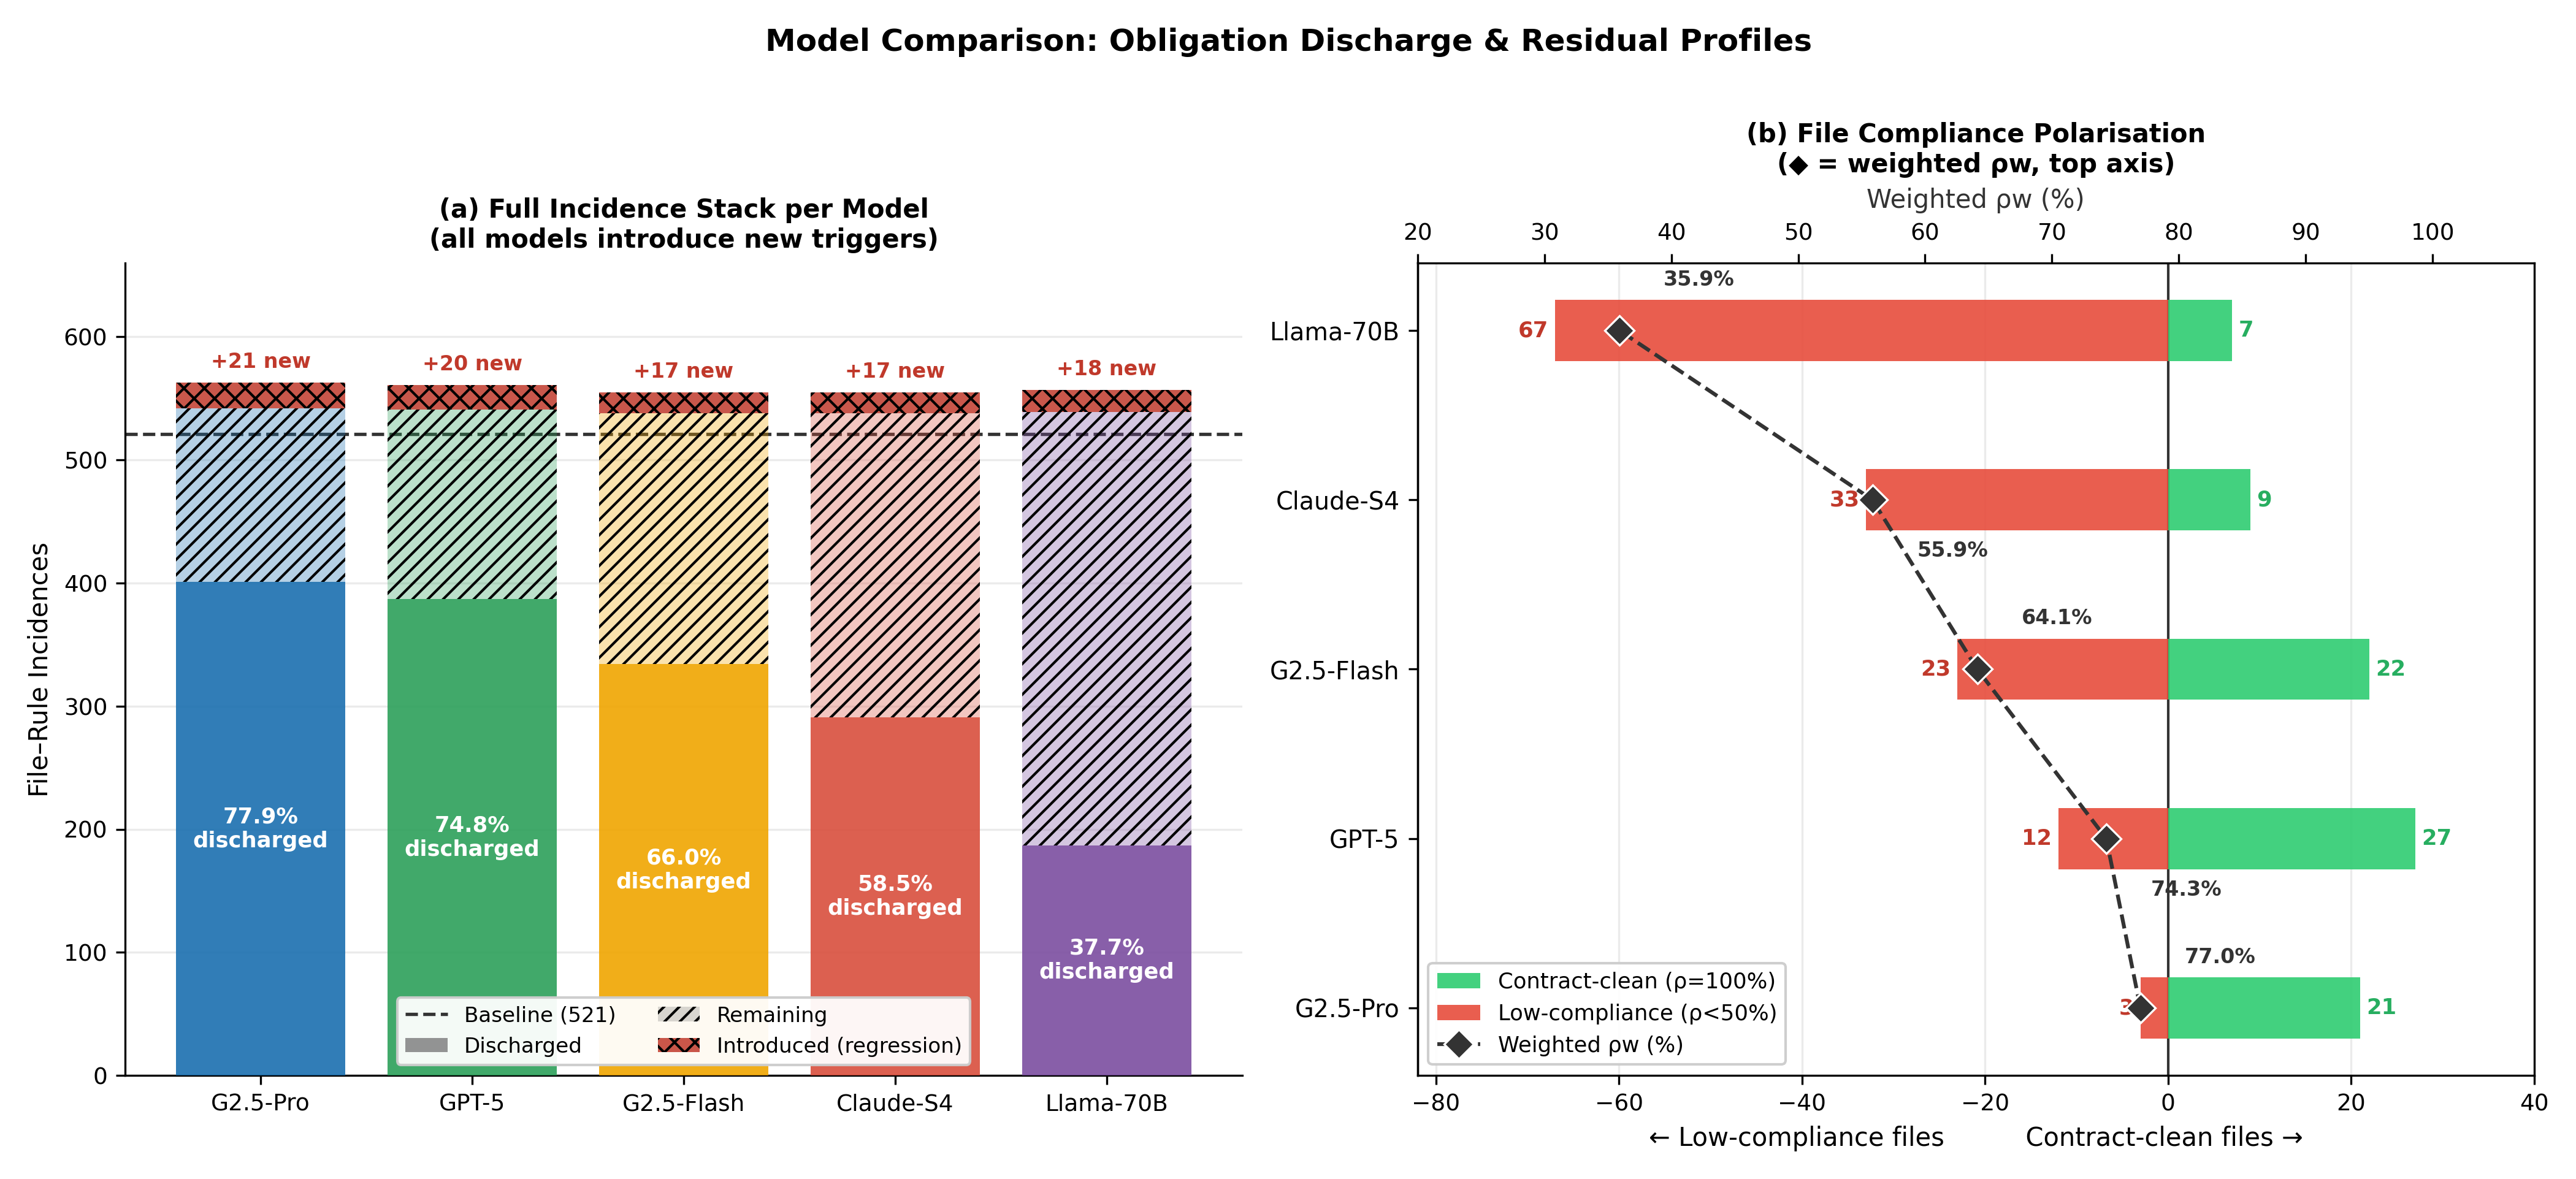
\includegraphics[width=\textwidth]{images/fig_models.png}
\caption{Pinned-contract compliance profiles across models.
  Bars show discharged and remaining obligations;
  auxiliary indicators summarise patch-volume closure and
  the concentration of remaining work.}
\label{fig:model_overview}
\end{figure*}


% =================================================================
%  SUBSECTION RQ1
% =================================================================
\subsection{RQ1: Migration progress under the pinned contract}
\label{sec:overall_results}

PCE reveals substantial variation in discharged and residual upgrade work
under a common all files denominator. Across 511 baseline file rule type
incidences, the contract aligned reference baseline (\emph{Rector applied})
discharges 503, yielding $\rho_w^{\mathrm{all}}=98.43\%$
(Table~\ref{tab:contract_discharge_summary}). This provides a strong,
though not perfect, reference point under the present ruleset.

For the LLM systems, weighted discharge ranges from 30.53\% to 72.80\%, with
2 to 19 contract clean files
(Table~\ref{tab:contract_discharge_summary}). Every system also introduces
new rule type incidences on analyzable migrated files. PCE therefore
separates discharged work, residual work, and newly introduced contract
visible regressions.


% =================================================================
%  SUBSECTION RQ2
% =================================================================
\subsection{RQ2: Resistant rules and migration demand}
\label{sec:size_results}

The remaining obligation space is structured rather than diffuse. Contract
progress declines as migration demand increases: discharge is lower on
larger files and on files with more baseline obligations
(Tables~\ref{tab:size_bin_discharge}, \ref{tab:correlation_results}).
Patch closure shows the same pattern, with unresolved work often
concentrated in a small number of files
(Table~\ref{tab:patch_closure},
Figure~\ref{fig:patch_concentration}).

Residual work is concentrated most clearly in PHP~8.x families
(Table~\ref{tab:php_family_discharge}). Rule level results show recurring
bottlenecks such as \texttt{NullToStrictStringFuncCallArg} and
\texttt{AddOverrideAttribute}, alongside introduced triggers such as
\texttt{ReadOnlyProperty}
(Table~\ref{tab:resistant_rules}). The main value of these results is
diagnostic: PCE localizes where automated migration remains least reliable
under a fixed policy.





% --- TWO side-by-side tables: size-bin discharge + patch closure --
\begin{table*}[t]
\centering
% ---- subtable A : size-bin discharge ----
\begin{minipage}[t]{0.56\textwidth}
\centering
\caption{Mean discharge (\%) by file-size bin .
  Parentheses: discharged / total incidences.}
\label{tab:size_bin_discharge}
\setlength{\tabcolsep}{4pt}
\renewcommand{\arraystretch}{1.18}
\resizebox{\linewidth}{!}{%
\begin{tabular}{L{3.0cm}C{1.8cm}C{1.8cm}C{1.7cm}C{2.0cm}}
\arrayrulecolor{hdrBlue}
\toprule[1.5pt]
\tophdr{Model} & \tophdr{Small} & \tophdr{Medium} & \tophdr{Large} & \tophdr{X-Large} \\
\midrule[1pt]
\rowcolor{rowA}
Gemini 2.5 Pro   & 77.6 {\tiny(77/99)} & 83.8 {\tiny(136/162)} & 74.8 {\tiny(105/141)} & 60.6 {\tiny(54/89)}  \\
\rowcolor{rowB}
GPT-5 Codex             & 75.9 {\tiny(76/99)}  & 75.9 {\tiny(111/146)} & 66.6 {\tiny(86/130)} & 45.1 {\tiny(24/53)}  \\
\rowcolor{rowA}
Gemini 2.5 Flash        & 71.5 {\tiny(70/99)}  & 67.0 {\tiny(104/153)} & 51.2 {\tiny(67/131)} & 41.8 {\tiny(32/76)}  \\
\rowcolor{rowB}
Claude Sonnet 4         & 65.8 {\tiny(60/91)}  & 69.3 {\tiny(111/158)} & 41.5 {\tiny(63/146)} & 38.3 {\tiny(38/104)} \\
\rowcolor{rowA}
Llama 3.3 70B   & 37.8 {\tiny(35/93)}  & 42.7 {\tiny(71/162)}  & 28.5 {\tiny(40/140)} & 11.9 {\tiny(10/90)}  \\
\bottomrule[1.5pt]
\end{tabular}}
\end{minipage}
\hfill
% ---- subtable B : patch closure ----
\begin{minipage}[t]{0.41\textwidth}
\centering
\caption{Patch-volume closure under the pinned contract (localization proxy).}
\label{tab:patch_closure}
\setlength{\tabcolsep}{4pt}
\renewcommand{\arraystretch}{1.18}
\resizebox{\linewidth}{!}{%
\begin{tabular}{L{2.8cm}C{1.3cm}C{1.3cm}C{1.4cm}R{2.0cm}}
\arrayrulecolor{hdrBlue}
\toprule[1.5pt]
\tophdr{System} & \tophdr{WDC} & \tophdr{MFDC} & \tophdr{Top-5} & \tophdr{Rem. lines} \\
\midrule[1pt]
\rowcolor{rowA}
\refrow{Rector (ref.)} & \refrow{95.1} & \refrow{98.2} & \refrow{91.4} & \refrow{1{,}109} \\
\midrule[0.4pt]
\rowcolor{rowB}
Gemini 2.5 Pro  & 71.9  & 76.9  & 50.7          & 5{,}826  \\
\rowcolor{rowA}
GPT-5 Codex            & 67.5         & 69.9         & 36.5   & 5{,}074  \\
\rowcolor{rowB}
Gemini 2.5 Flash       & 60.7         & 64.8         & 43.5          & 7{,}620  \\
\rowcolor{rowA}
Claude Sonnet 4        & 57.8         & 62.8         & 40.3          & 9{,}411  \\
\rowcolor{rowB}
Llama 3.3 70B  & 36.7 & 42.3 & 39.4          & 12{,}342 \\
\bottomrule[1.5pt]
\end{tabular}}
\end{minipage}
\end{table*}

% =================================================================
%  FIGURE — Patch concentration  (inline with RQ2 text)
% =================================================================
\begin{figure}[t]
\centering
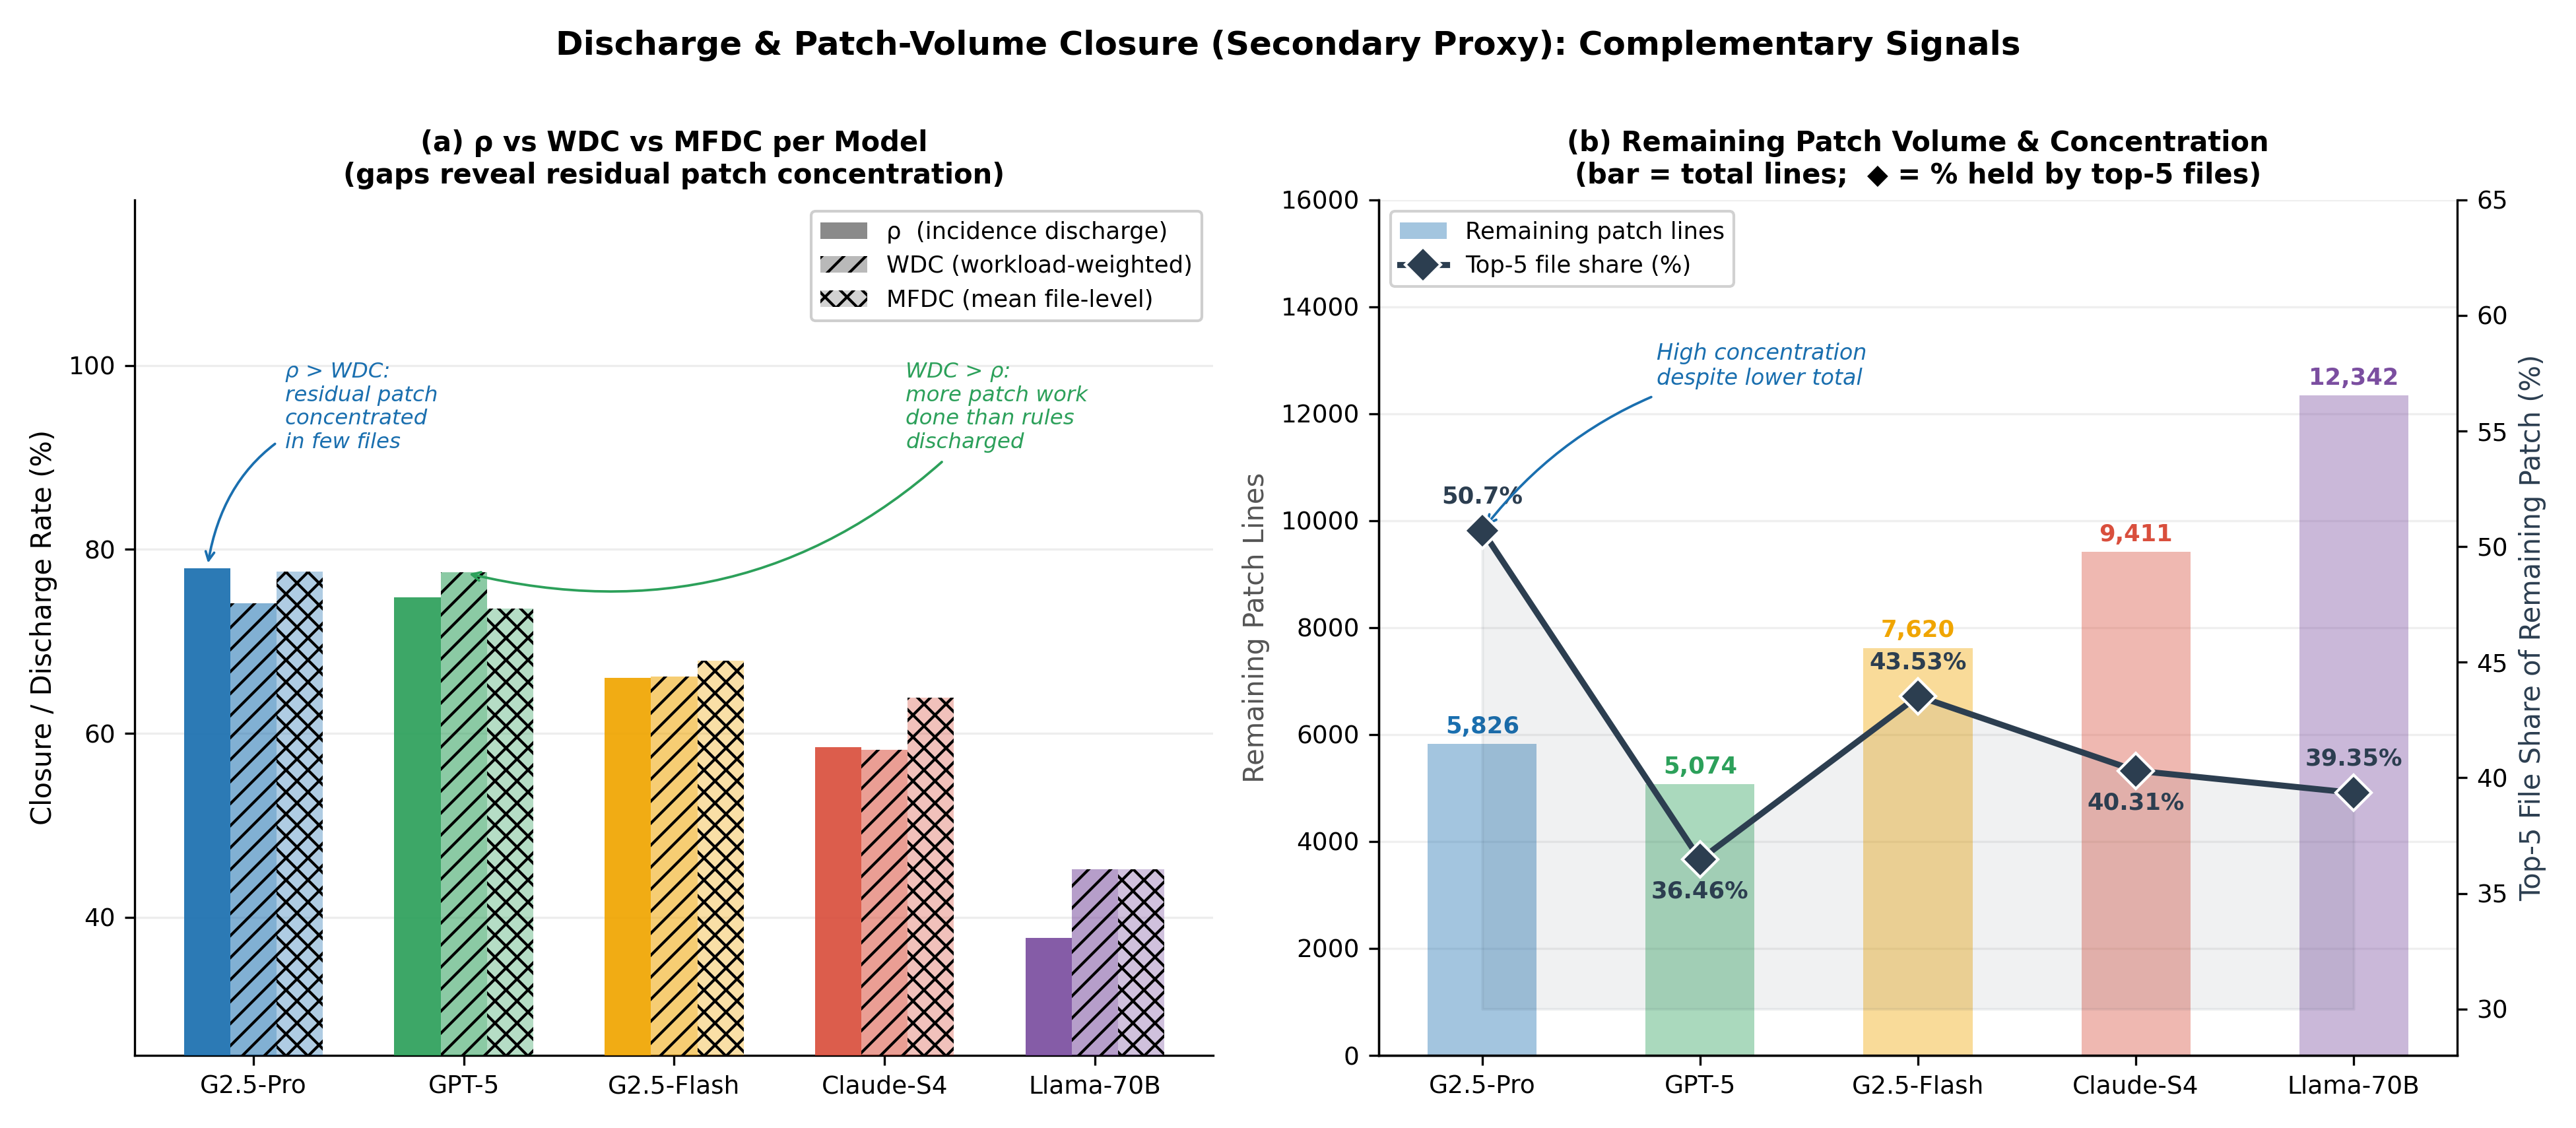
\includegraphics[width=\columnwidth]{images/fig_patch.png}
\caption{Remaining patch volume and concentration across models.
  Bars show total remaining patch lines;
  markers show the share concentrated in the top files.}
\label{fig:patch_concentration}
\end{figure}



% --- TWO side-by-side tables: PHP-family discharge + correlation --
\begin{table*}[t]
\centering
\begin{minipage}[t]{0.54\textwidth}
\centering
\caption{Discharged obligations by PHP family (analyzable files only).}
\label{tab:php_family_discharge}
\setlength{\tabcolsep}{4pt}
\renewcommand{\arraystretch}{1.18}
\resizebox{\linewidth}{!}{%
\begin{tabular}{L{3.2cm}C{2.6cm}C{2.6cm}C{2.6cm}}
\arrayrulecolor{hdrBlue}
\toprule[1.5pt]
\tophdr{Model} & \tophdr{PHP 5.x} & \tophdr{PHP 7.x} & \tophdr{PHP 8.x} \\
\midrule[1pt]
\rowcolor{rowA}
Gemini 2.5 Pro  & 143/149 (95.97\%) & 114/126 (90.48\%) & 115/216 (53.24\%) \\
\rowcolor{rowB}
GPT-5 Codex            & 126/133 (94.74\%)        & 88/106 (83.02\%)         & 83/189 (43.92\%)  \\
\rowcolor{rowA}
Gemini 2.5 Flash       & 116/137 (84.67\%)        & 97/120 (80.83\%)         & 60/202 (29.70\%)  \\
\rowcolor{rowB}
Claude Sonnet 4        & 109/150 (72.67\%)        & 92/129 (71.32\%)         & 71/220 (32.27\%)  \\
\rowcolor{rowA}
Llama 3.3 70B  & 87/145 (60.00\%) & 53/125 (42.40\%) & 16/215 (7.44\%)  \\
\bottomrule[1.5pt]
\end{tabular}}
\end{minipage}
\hfill
\begin{minipage}[t]{0.42\textwidth}
\centering
\caption{Pearson correlation between demand proxies and type-level
  discharge on each model's analyzable migrated files.}
\label{tab:correlation_results}
\setlength{\tabcolsep}{4pt}
\renewcommand{\arraystretch}{1.18}
\resizebox{\linewidth}{!}{%
\begin{tabular}{L{3.4cm}C{2.0cm}C{2.0cm}}
\arrayrulecolor{hdrBlue}
\toprule[1.5pt]
\tophdr{Model} & \tophdr{$r(\mathrm{LOC},\rho_i)$} & \tophdr{$r(O_i,\rho_i)$} \\
\midrule[1pt]
\rowcolor{rowA}
Gemini 2.5 Flash       & $-$0.453 & $-$0.300 \\
\rowcolor{rowB}
Gemini 2.5 Pro         & $-$0.405 & $-$0.212 \\
\rowcolor{rowA}
GPT-5 Codex            & $-$0.337 & $-$0.236 \\
\rowcolor{rowB}
Claude Sonnet 4        & $-$0.459 & $-$0.267 \\
\rowcolor{rowA}
Llama 3.3 70B          & $-$0.356 & $-$0.204 \\
\bottomrule[1.5pt]
\end{tabular}}
\end{minipage}
\end{table*}

% --- Resistant rules table (full width) --------------------------
\begin{table*}[t]
\centering
\caption{Most resistant Rector upgrade rules across models (file-level trigger breadth).
  \emph{Orig.}\ = benchmark files in which the rule triggers.
  For Orig.\,$>$0: \% of file-level triggers discharged.
  For Orig.\,=\,0: introduced file-level triggers ($+k$).}
\label{tab:resistant_rules}
\setlength{\tabcolsep}{4pt}
\renewcommand{\arraystretch}{1.18}
\resizebox{\textwidth}{!}{%
\begin{tabular}{%
  L{3.6cm}          % Rule
  C{0.9cm}          % PHP ver
  L{4.4cm}          % Challenge
  C{1.0cm}          % Orig
  C{1.3cm}          % Pro
  C{1.3cm}          % Flash
  C{1.3cm}          % GPT-5
  C{1.3cm}          % Claude
  C{1.3cm}%         % LLaMA
}
\arrayrulecolor{hdrBlue}
\toprule[1.5pt]
\tophdr{Rule} &
\tophdr{PHP} &
\tophdr{Migration Challenge} &
\tophdr{Orig.} &
\tophdr{Pro} &
\tophdr{Flash} &
\tophdr{GPT-5} &
\tophdr{Claude} &
\tophdr{LLaMA} \\
\midrule[1pt]
% --- group header -----------------------------------------------
\multicolumn{9}{l}{\subhdr{\quad Type strictness \& null-safety}} \\
\rowcolor{rowA}
\texttt{\small NullToStrict\-Func\-Call\-Arg} & 8.1 &
  Null-safety across non-local flow & 81 & 27 & 32 & 48 & 11 & 14 \\
\rowcolor{rowB}
\texttt{\small Stringable\-For\-ToString}      & 8.0 &
  Interface decl.\ for \texttt{\_\_toString()} &  8 & 13 & 13 &  0 &  0 &  0 \\
\midrule[0.4pt]
\multicolumn{9}{l}{\subhdr{\quad Modern callable \& attribute syntax (near-zero discharge)}} \\
\rowcolor{rowA}
\texttt{\small FirstClass\-Callable}           & 8.1 &
  Callable vs.\ string-literal ambiguity & 13 & 31 & 23 & 15 &  8 &  8 \\
\rowcolor{rowB}
\texttt{\small AddOverride\-Attribute}         & 8.3 &
  Cross-file hierarchy reasoning         &  7 & 29 & 14 & 29 & 14 & 14 \\
\rowcolor{rowA}
\texttt{\small AddType\-To\-Const}             & 8.3 &
  Type decls.\ requiring global inference &  0 & +5 & +1 & +1 & +2 & +1 \\
\midrule[0.4pt]
\multicolumn{9}{l}{\subhdr{\quad Introduced ``modern'' constructs (over-eager / regression risk)}} \\
\rowcolor{rowB}
\texttt{\small ReadOnly\-Property}             & 8.1 &
  Single-assignment detection (FP risk)  &  0 & +8 & +4 & +4 & +5 & +9 \\
\bottomrule[1.5pt]
\end{tabular}}
\end{table*}


% =================================================================
%  SUBSECTION RQ3 — Validity, preservation, loadability
% =================================================================
\subsection{RQ3: Contract progress and complementary diagnostics}
\label{sec:syntax_and_structure}

Contract progress and robustness align only partially
(Figure~\ref{fig:robustness}). All LLM systems introduce new syntax
failures
(Table~\ref{tab:syntax_model_results}), showing that substantial discharge
does not by itself guarantee a parsable result set.

Structural diagnostics add a second qualification
(Table~\ref{tab:completeness_model_results}). Signature stability remains
high, but deeper preservation varies more noticeably. The loadability
sentinel shows the same partial alignment: new failures on the execution
slice range from 14.5\% to 32.7\%
(Table~\ref{tab:runtime_slice_results}). PCE is therefore informative about
policy grounded migration progress, but it must be read with orthogonal
diagnostics.

% --- TWO side-by-side tables: syntax + loadability ---------------
\begin{table*}[t]
\centering
\begin{minipage}[t]{0.50\textwidth}
\centering
\caption{Syntax validity (\texttt{php -l}, PHP 8.3) over 100 files.
  \textbf{New} = hard regressions (Pass$\to$Fail).
  NR-valid = Both valid + Fixed.}
\label{tab:syntax_model_results}
\setlength{\tabcolsep}{4pt}
\renewcommand{\arraystretch}{1.18}
\resizebox{\linewidth}{!}{%
\begin{tabular}{L{3.2cm}C{0.9cm}C{1.2cm}C{1.1cm}C{1.5cm}C{1.5cm}C{1.3cm}}
\arrayrulecolor{hdrBlue}
\toprule[1.5pt]
\tophdr{System} &
\tophdr{New$\downarrow$} &
\tophdr{Migr Err} &
\tophdr{Fixed$\uparrow$} &
\tophdr{Both valid} &
\tophdr{NR-valid$\uparrow$} &
\tophdr{Orig Err} \\
\midrule[1pt]
\rowcolor{rowA}
\refrow{Rector (ref.)} & \refrow{1} & \refrow{1} & \refrow{9} & \refrow{90} & \refrow{99} & \refrow{9} \\
\midrule[0.4pt]
\rowcolor{rowB}
Gemini 2.5 Pro  & 11 & 13 & 7 & 80 & 87 & 9 \\
\rowcolor{rowA}
Claude Sonnet 4 & 11 & 12 & 8 & 80 & 88 & 9 \\
\rowcolor{rowB}
GPT-5 Codex            & 14 & 18 & 5 & 77 & 82 & 9 \\
\rowcolor{rowA}
Llama 3.3 70B          & 16 & 23 & 2 & 75 & 77 & 9 \\
\rowcolor{rowB}
Gemini 2.5 Flash & 18 & 20 & 7 & 73 & 80 & 9 \\
\bottomrule[1.5pt]
\end{tabular}}
\end{minipage}
\hfill
\begin{minipage}[t]{0.46\textwidth}
\centering
\caption{Loadability tripwire on the 55-file execution slice (\%).
  \textbf{Regress} = new failures (Pass$\to$Fail). $\rho$ = mean discharge.}
\label{tab:runtime_slice_results}
\setlength{\tabcolsep}{4pt}
\renewcommand{\arraystretch}{1.18}
\resizebox{\linewidth}{!}{%
\begin{tabular}{L{3.2cm}C{1.5cm}C{1.2cm}C{1.2cm}C{1.2cm}}
\arrayrulecolor{hdrBlue}
\toprule[1.5pt]
\tophdr{System} &
\tophdr{Regress$\downarrow$} &
\tophdr{Pass$\uparrow$} &
\tophdr{$\rho$} &
\tophdr{Other} \\
\midrule[1pt]
\rowcolor{rowA}
\refrow{Rector (ref.)}  & \refrow{12.7} & \refrow{83.6} & \refrow{98.3} & \refrow{3.6} \\
\midrule[0.4pt]
\rowcolor{rowB}
Claude Sonnet 4  & 14.5  & 80.0 & 57.0 & 5.5 \\
\rowcolor{rowA}
GPT-5 Codex             & 16.4  & 78.2 & 58.7 & 5.5 \\
\rowcolor{rowB}
Gemini 2.5 Pro          & 21.8  & 72.7 & 74.6 & 5.5 \\
\rowcolor{rowA}
Llama 3.3 70B           & 21.8  & 69.1 & 36.2 & 9.1 \\
\rowcolor{rowB}
Gemini 2.5 Flash& 32.7 & 60.0 & 53.5 & 7.3 \\
\bottomrule[1.5pt]
\end{tabular}}
\end{minipage}
\end{table*}

% --- Structural preservation (full width) -----------------------
\begin{table*}[t]
\centering
\caption{Structural preservation and anti-gaming diagnostics over 100 files.
  Line/Func/Class/Struct are retention ratios ($>$100\% indicates expansion).
  Body/SigStab/TrivialStub/EmptyBody are computed on matched declarations (80/100).}
\label{tab:completeness_model_results}
\setlength{\tabcolsep}{4pt}
\renewcommand{\arraystretch}{1.18}
\resizebox{\textwidth}{!}{%
\begin{tabular}{%
  L{3.4cm}
  C{1.4cm}C{1.3cm}C{1.3cm}C{1.3cm}C{1.3cm}C{1.4cm}C{1.5cm}C{1.5cm}%
}
\arrayrulecolor{hdrBlue}
\toprule[1.5pt]
\tophdr{System} &
\tophdr{Line (\%)} &
\tophdr{Func (\%)} &
\tophdr{Class (\%)} &
\tophdr{Struct (\%)} &
\tophdr{Body (\%)} &
\tophdr{SigStab} &
\tophdr{Trivial\-Stub} &
\tophdr{Empty\-Body} \\
\midrule[1pt]
\rowcolor{rowA}
\refrow{Rector (ref.)}  &  \refrow{98.87} &  \refrow{99.91} & \refrow{100.00} & \refrow{97.69} & \refrow{95.73} & \refrow{1.000} & \refrow{0.082} & \refrow{0.038} \\
\midrule[0.4pt]
\rowcolor{rowB}
Claude Sonnet 4         &  97.37 & 102.16 & 100.00 & 95.23 & 91.95 & 0.996 & 0.123 & 0.035 \\
\rowcolor{rowA}
GPT-5 Codex             & 105.40 &  96.03 &  99.00 & 94.02 &       93.16  &       0.988  & 0.116 & 0.027 \\
\rowcolor{rowB}
Gemini 2.5 Flash        &  95.85 &  96.57 &  99.00 & 91.39 &       89.39  &       0.989  & 0.114 & 0.037 \\
\rowcolor{rowA}
Gemini 2.5 Pro   & 100.04 &  97.42 &  99.50 & 90.20 & 80.20 & 0.979 & 0.115 & 0.024 \\
\rowcolor{rowB}
Llama 3.3 70B           &  97.12 &  98.33 &  99.00 & 89.96 &       93.67  &       0.990  & 0.106 & 0.018 \\
\bottomrule[1.5pt]
\end{tabular}}
\end{table*}

% --- Robustness figure ------------------------------------------
\begin{figure*}[t]
\centering
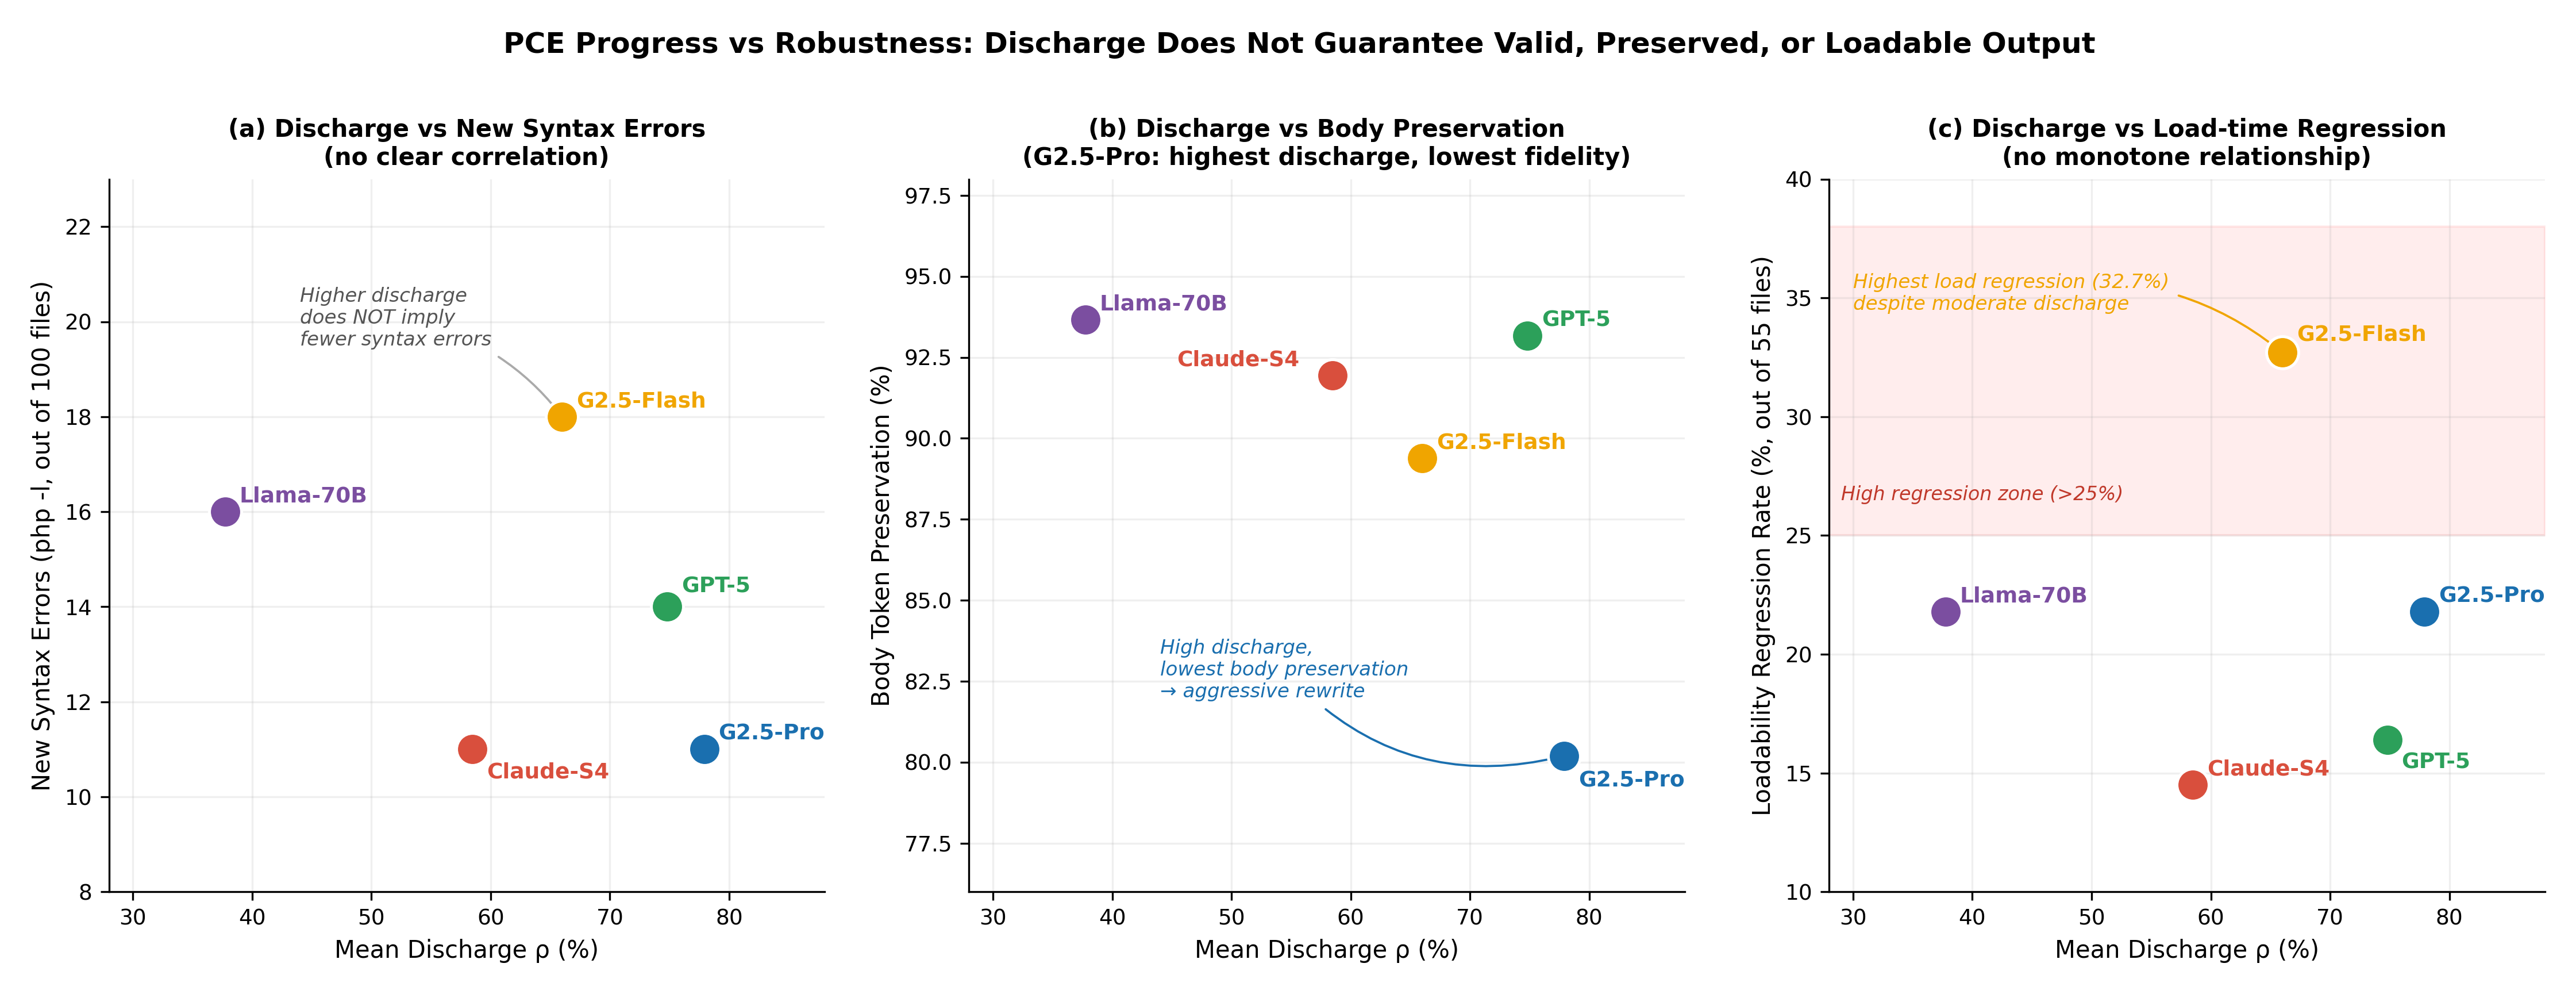
\includegraphics[width=\textwidth]{images/fig_validity.png}
\caption{Contract discharge versus robustness diagnostics across models.
  Higher contract compliance does not necessarily imply fewer syntax
  errors, stronger structural preservation, or better loadability.}
\label{fig:robustness}
\end{figure*}


% =================================================================
%  SUBSECTION RQ4 — PHPCompatibility
% =================================================================
\subsection{RQ4: Cross instrument triangulation with PHPCompatibility}
\label{sec:phpcompat_results}

PCE and PHPCompatibility provide related but non identical views of
migration progress
(Table~\ref{tab:phpcompat_validation}). Some systems improve under both
instruments, but the magnitude of improvement and the relative ordering do
not fully coincide.

This divergence is methodological rather than contradictory. PCE measures
discharged obligations under a pinned Rector contract, whereas
PHPCompatibility reports issues under an independent rule set. Read
together, they show that evaluation conclusions depend in part on the
instrument used.

% --- PHPCompatibility table (full width) ------------------------
\begin{table*}[t]
\centering
\caption{PHPCS+PHPCompatibility results (\texttt{testVersion=8.3}) with
  concentration diagnostics over 100 files.
  Issues = errors + warnings; Clean = zero-issue files;
  $\Delta$Issues relative to original benchmark.}
\label{tab:phpcompat_validation}
\setlength{\tabcolsep}{4pt}
\renewcommand{\arraystretch}{1.18}
\resizebox{\textwidth}{!}{%
\begin{tabular}{%
  L{3.2cm}
  R{1.3cm}@{\hspace{3pt}}
  R{1.4cm}@{\hspace{3pt}}
  R{1.1cm}@{\hspace{3pt}}
  R{1.1cm}@{\hspace{3pt}}
  R{1.4cm}@{\hspace{3pt}}
  R{1.0cm}@{\hspace{3pt}}
  R{1.2cm}@{\hspace{3pt}}
  L{2.8cm}@{\hspace{3pt}}
  R{1.2cm}%
}
\arrayrulecolor{hdrBlue}
\toprule[1.5pt]
\tophdr{System} &
\tophdr{Issues$\downarrow$} &
\tophdr{$\Delta$Issues} &
\tophdr{Err$\downarrow$} &
\tophdr{Warn$\downarrow$} &
\tophdr{Clean$\uparrow$} &
\tophdr{P95$\downarrow$} &
\tophdr{Top-5} &
\tophdr{Dom.\ code} &
\tophdr{Share} \\
\midrule[1pt]
\rowcolor{rowA}
\refrow{Original}          & \refrow{255} & \refrow{0}    & \refrow{45}  & \refrow{210} & \refrow{76 (76\%)} & \refrow{14} & \refrow{63.9\%} & \texttt{\scriptsize CurlyBraceAccess} & \refrow{56.1\%} \\
\rowcolor{rowB}
\refrow{Rector (ref.)}     & \refrow{48}  & \refrow{$-$207} & \refrow{27}  & \refrow{21}  & \refrow{88 (88\%)} & \refrow{3}  & \refrow{77.1\%} & \texttt{\scriptsize mysql\_removed}   & \refrow{43.8\%} \\
\midrule[0.6pt]
\rowcolor{rowA}
Gemini 2.5 Pro  & 10   & $-$245 & 9   & 1  & 97 (97\%) & 0 & 100.0\%& \texttt{\scriptsize mysql\_removed}   & 70.0\%  \\
\rowcolor{rowB}
Claude Sonnet 4        & 39          & $-$216          & 27         & 12        & 90 (90\%)        & 2        & 84.6\%         & \texttt{\scriptsize mysql\_removed}   & 53.8\%  \\
\rowcolor{rowA}
Gemini 2.5 Flash       & 139         & $-$116          & 125        & 14        & 88 (88\%)        & 2        & 93.5\%         & \texttt{\scriptsize this\_outside}    & 76.3\%  \\
\rowcolor{rowB}
GPT-5 Codex            & 181         & $-$74           & 172        &  9        & 91 (91\%)        & 1        & 97.8\%         & \texttt{\scriptsize this\_outside}    & 87.3\%  \\
\rowcolor{rowA}
Llama 3.3 70B  & 484 & $+$229  & 377& 107& 85 (85\%)& 6& 95.2\%         & \texttt{\scriptsize this\_outside}    & 71.5\%  \\
\bottomrule[1.5pt]
\end{tabular}}
\end{table*}


% =================================================================
%  SUMMARY
% =================================================================
\subsection{Summary}
\label{sec:tradeoffs}

Taken together, the results support the role of PCE as a policy grounded
measurement layer rather than a stand alone correctness signal. Under the
pinned contract, PCE reveals substantial variation in discharged migration
work, with unresolved obligations concentrated in PHP~8.x families.
Complementary diagnostics then delimit what that progress does and does not
imply about syntax, preservation, loadability, and independent
compatibility.


\section{Threats to Validity}
\label{sec:threats}

\paragraph{Construct validity}
PCE measures modernization against a fixed static-analysis policy.
The policy is a pinned Rector configuration.
Our primary metric uses file-level rule-type incidence.
This signal is tool-native and stable across runs.
It supports reproducible comparison.
However, incidence ignores within-file frequency and severity.
Discharge is conservative.
A rule type counts as resolved only when it no longer triggers in the file.

Patch volume closure is a secondary proxy.
It uses dry-run changed-line counts.
Diff size can change due to formatting or restructuring.
It is not a measure of developer effort.
We reduce this risk by using the same pinned contract for all systems and by avoiding extra formatting passes.

Contract metrics can be inflated by omission or degenerate rewrites.
We therefore interpret discharge with diagnostics.
We report syntax validity, structural preservation and anti-degeneracy signals, introduced-rule regressions, a loadability sentinel, and PHPCompatibility.

\paragraph{Internal validity}
Results can be affected by orchestration.
Context limits, chunk boundaries, extraction failures, and provider APIs can change outputs.
We reduce these effects by fixing prompts, chunking policy, and decoding settings where supported.
We use deterministic parsing and reconstruction.
We surface failures instead of repairing outputs.

\paragraph{External validity}
We study PHP version migration on a WordPress-derived benchmark.
The benchmark is coverage-optimized for the obligation space induced by the pinned policy.
It is not representative of WordPress file frequencies.
Results therefore reflect performance under this contract and this sampling strategy.
Other projects and other pinned pipelines may induce different obligation spaces.
The PCE methodology should still apply, but outcomes may differ.

\paragraph{Reliability and reproducibility}
Tool versions and configurations are pinned.
All artifacts are logged.
Still, LLM outputs can vary due to nondeterminism, missing seeds, and provider-side updates.
The loadability sentinel is environment dependent.
We interpret it only as a directional regression signal (orig.\ pass $\rightarrow$ migrated fail) under the same harness.

\section{Conclusion and Future Work}
\label{sec:conclusion}

We introduced \emph{Pinned Contract Evaluation (PCE)}.
PCE evaluates automated code modernization against an explicit upgrade policy.
The policy is a pinned static-analysis contract.
PCE measures progress in the induced obligation space.
We score incidence-level obligation discharge and track contract-visible regressions ($I_i, \Delta_i$).
We also report patch volume closure as a diff-magnitude proxy.
We interpret these metrics with syntax checks, structural preservation diagnostics, PHPCompatibility, and a regression-oriented loadability sentinel.

\paragraph{Findings}
On a coverage-optimized WordPress-derived benchmark, PHP~5.x and 7.x obligations discharge more often than PHP~8.x obligations.
Residual work concentrates in later-version rules and a small set of difficult files.
Contract discharge does not always track robustness.
Cross-instrument signals can also diverge.
Different policies capture different upgrade properties.
Overall, PCE localizes what was fixed and what remains under a fixed contract.

\paragraph{Future work}
We plan to build additional pinned pipelines that represent alternative upgrade policies.
We will extend to other ecosystems and codebases.
We will add stronger execution-based validation when realistic harnesses exist.
We also plan feedback-driven post-editing guided by residual obligation profiles.



\bibliographystyle{IEEEtran}
\bibliography{references}


\clearpage
\appendices


% Appendix-style algorithm numbering (A1, A2, ...)
\setcounter{algorithm}{0}
\renewcommand{\thealgorithm}{A\arabic{algorithm}}

\newenvironment{appalgorithm}[2]{%
  \refstepcounter{algorithm}\label{#2}%
  \Needspace{10\baselineskip}% avoid splitting header from first lines
  \par\medskip
  \noindent\hrule height 0.4pt\relax
  \vspace{0.35em}
  \noindent\textbf{Algorithm \thealgorithm.} #1\par
  \vspace{0.35em}
  \small
}{%
  \par\normalsize
  \vspace{0.35em}
  \noindent\hrule height 0.4pt\relax
  \par\medskip
}

% ============================================================
% Appendix A
% ============================================================
\section{Benchmark Construction and Chunking Algorithms}
\label{app:benchmark_algorithms}

\noindent This appendix summarizes three procedures used in benchmark construction and context-bounded migration:
(i) relevance scoring, (ii) constraint-aware selection, and (iii) PHP-aware smart chunking.

% ------------------------------------------------------------
\subsection{Benchmark construction}
\label{app:benchmark_construction}

\paragraph{Relevance scoring.}
We score candidate files by contract-triggered rule activity and migration relevance signals.

\begin{appalgorithm}{File scoring for migration relevance under the pinned contract.}{alg:file_scoring}
\begin{algorithmic}[1]
  \Require file with $LOC$, $V$ (\texttt{php\_version\_changes}), and triggered rules $R$
  \Ensure relevance score $s$
  \State $s \gets 10 \cdot |R| + 5 \cdot V$
  \If{$100 \le LOC \le 2000$}
    \State $s \gets s + 20$
  \ElsIf{$LOC > 2000$}
    \State $s \gets s - 0.01 \cdot (LOC - 2000)$
  \EndIf
  \State $s \gets s + 8 \cdot \left|\{\text{PHP rule families covered by } R\}\right|$
  \State $s \gets s + \textsc{ImportantRuleBonus}(R)$
  \State \Return $s$
\end{algorithmic}
\end{appalgorithm}

\paragraph{Constraint-aware selection.}
We select 100 files while enforcing full rule coverage as the hard constraint.

\begin{appalgorithm}{Constraint-aware selection of 100 files with full rule coverage.}{alg:selection_engine}
\begin{algorithmic}[1]
  \Require summary table, rule metadata, size bins, target counts $T$
  \Ensure selected file set $S$
  \State group files by size category
  \State compute score for each file using Algorithm~\ref{alg:file_scoring}
  \ForAll{size categories $c$}
    \State select top $T[c]$ files by score into $S$
  \EndFor
  \State $S \gets \textsc{EnsureRuleCoverage}(S)$
    \Comment{May add files outside bin quotas; coverage is the hard constraint}
  \If{$|S| > 100$}
    \State trim lowest-scoring files if coverage is preserved
  \ElsIf{$|S| < 100$}
    \State add highest-scoring remaining files until $|S| = 100$
  \EndIf
  \State \Return $S$
\end{algorithmic}
\end{appalgorithm}

% ------------------------------------------------------------
\subsection{PHP-aware chunking for bounded-context migration}
\label{app:chunking}

\paragraph{Smart chunking.}
We split long PHP files into bounded-context segments while attempting to avoid mid-function splits under a fixed policy.

\begin{appalgorithm}{PHP-aware smart chunking.}{alg:smart_chunking}
\begin{algorithmic}[1]
\Require $code$ (PHP source string), $chunk\_size$ (target lines), $MAX\_EXTENSION$ (max extension in lines)
\Ensure $chunks$ (list of records $\{start\_line,end\_line,actual\_size,total\_lines,code\}$)
\State $lines \gets \Call{Split}{code,\ "\backslash n"}$
\State $total \gets |lines|$
\If{$total \le chunk\_size$}
  \State \Return $[\{1,total,total,total,code\}]$
\EndIf
\State $boundaries \gets \Call{FindFunctionBoundaries}{code}$
\Comment{Tokenizer-guided detection via \texttt{token\_get\_all} when available; regex fallback; end lines approximated via brace matching}
\State $chunks \gets [\ ]$
\State $current \gets 0$
\While{$current < total$}
  \State $initial\_end \gets \min(current + chunk\_size - 1,\ total - 1)$
  \State $final\_end \gets initial\_end$
  \State $relevant \gets \{f \in boundaries \mid (current \le f.start \le initial\_end)\ \lor\ (f.start < current \land f.end \ge current)\}$
  \ForAll{$f \in relevant$}
    \If{$f.end \le initial\_end + MAX\_EXTENSION$}
      \State $final\_end \gets \max(final\_end, f.end_prof)$
      \State $final\_end \gets \max(final\_end, f.end)$
    \EndIf
  \EndFor
  \State $chunk\_code \gets \Call{Join}{lines[current..final\_end],\ "\backslash n"}$
  \State append $\{current+1,final\_end+1,(final\_end-current+1),total,chunk\_code\}$ to $chunks$
  \State $current \gets final\_end + 1$
\EndWhile
\State \Return $chunks$
\end{algorithmic}
\end{appalgorithm}

% ============================================================
% Appendix B
% ============================================================

\section{Prompt Templates}
\label{app:prompt_templates}

We use prompting shared across models, with whole-file and chunk-segment variants.
In both templates, \texttt{\{code\}} is replaced with the input PHP text.

\subsection{Whole-file prompt}
\noindent\begin{Verbatim}[breaklines=true,breakanywhere=true,fontsize=\footnotesize]
You are a senior PHP developer with expertise in legacy code modernization.
Your task is to migrate this legacy PHP code up to PHP 8.3 standards using modern syntax and features while maintaining functional equivalence.

Please migrate the following PHP code up to PHP 8.3 standards:

{code}

Your response should follow this EXACT format:

// MIGRATION_START
[your migrated PHP code here]
// MIGRATION_END

CRITICAL FORMATTING REQUIREMENT:
- Place the MIGRATION_START marker BEFORE the opening <?php tag
- Place the MIGRATION_END marker AFTER the closing PHP code
- Do NOT place these markers inside the PHP code itself

Provide only the migrated PHP code with the markers placed correctly outside the PHP code block, no additional commentary.
\end{Verbatim}

\subsection{Chunk-segment prompt}
The placeholders \texttt{\{filename\}}, \texttt{\{start\_line\}}, \texttt{\{end\_line\}}, \texttt{\{total\_lines\}}, \texttt{\{chunk\_number\}}, and \texttt{\{total\_chunks\}} are filled from the chunk metadata.

\noindent\begin{Verbatim}[breaklines=true,breakanywhere=true,fontsize=\footnotesize]
You are a senior PHP developer with expertise in legacy code modernization.
Your task is to migrate this PARTIAL SEGMENT of a larger PHP file up to PHP 8.3 standards using modern syntax and features.

CONTEXT:
- Original file: {filename}
- Processing lines: {start_line} to {end_line} (of {total_lines} total lines)
- This is chunk {chunk_number} of {total_chunks}

CRITICAL INSTRUCTIONS FOR PARTIAL CODE SEGMENTS:
1. This is ONLY a SEGMENT of a larger file - DO NOT try to complete it
2. keep the original opening <?php tag if present. if the segment does not start with <?php, DO NOT add one
3. keep the original closing ?> tag if present. If the segment does not end with ?>, DO NOT add one
4. keep the original closing braces }} if present. DO NOT add any closing braces that are not in the original segment
5. keep the original opening braces {{ if present. DO NOT add any opening braces that are not in the original segment
6. DO NOT try to complete class definitions, function definitions, or any code structures
7. Preserve the EXACT START and END boundaries of the provided code segment

WARNING: Adding extra braces that are not in the original segment or completing code structures will break the reconstruction process!

Please modernize ONLY the following PHP code segment up to PHP 8.3 standards:

{code}

Your response should follow this EXACT format:

// MIGRATION_START
[your modernized code segment here - exactly as provided, no additions]
// MIGRATION_END

CRITICAL FORMATTING REQUIREMENT:
- Place the MIGRATION_START marker BEFORE the code segment
- Place the MIGRATION_END marker AFTER the code segment
- Do NOT place these markers inside the PHP code itself

Migrate only the provided code segment. Do not add any missing parts or try to complete incomplete structures.
\end{Verbatim}

% ============================================================
% Appendix C
% ============================================================
\section{Loadability Tripwire Slice Specification}
\label{app:runtime_validation}

This appendix documents the \emph{isolated, stubbed loadability tripwire} used on an execution slice to surface harness-visible load-time failures after migration.
It specifies the execution environment, harness bootstrap, slice accounting, outcome taxonomy, and diagnostic coverage.

\subsection{Scope and interpretation}
This signal is \emph{harness-dependent} and is not an integration test or an end-to-end correctness guarantee.
We interpret it primarily as a \emph{regression tripwire}: \emph{New failure} (Orig.\ Pass $\rightarrow$ Migr.\ Fail).
Unless otherwise stated, all percentages are computed over the full slice size $N_{\mathrm{rt}}=55$ (no files are excluded).
We therefore treat this tier as a \emph{within-harness regression detector} whose purpose is to flag newly introduced load-time failures under identical conditions.

\subsection{Regression definition and harness-scoped interpretation}
A \textbf{regression} is defined as a file that loaded successfully in the original snapshot (under PHP 8.3.22 + stubs) but fails to load after migration.
These are harness-visible include-time failures: parse errors, fatal errors, uncaught exceptions, and missing-symbol errors that prevent \texttt{require\_once} from completing.

Observed regression counts across the slice ($N_{\mathrm{rt}}=55$):

\begin{center}
\footnotesize
\begin{tabular}{@{}lrr@{}}
\toprule
\textbf{Model} & \textbf{Regressions} & \textbf{Regression Rate} \\
\midrule
Rector Baseline & 7 & 12.7\% \\
Claude Sonnet 4 & 8 & 14.5\% \\
GPT-5 Codex & 9 & 16.4\% \\
Llama 3.3 70B & 12 & 21.8\% \\
Gemini 2.5 Pro & 12 & 21.8\% \\
Gemini 2.5 Flash & 18 & 32.7\% \\
\bottomrule
\end{tabular}
\end{center}

\noindent\textbf{Interpretation scope.}
These failures represent \emph{harness-visible include-time defects}---i.e., the file cannot be included without a fatal condition under the tripwire harness---but they are detected under isolated-stub conditions, not full application bootstrap.
Accordingly, the harness does not validate behavioral correctness, API contracts, or end-to-end functionality; it detects only include-time failures.
A file that passes this tripwire may still contain behavioral regressions; conversely, some files that fail may succeed under full WordPress initialization.
We treat \emph{New failure} counts as a \emph{lower bound} on migration breakage under the harness: they surface include-time breaks (e.g., syntax errors, missing symbols, invalid includes, or signature/parameter drops that trigger immediate fatals) that static contract discharge may not detect, but do not capture semantic or integration-level issues.

%------------------------------------------------------------------------------
\subsection{Execution environment}
\label{appendix:exec-env}

All tripwire checks are performed under a fixed environment for repeatability.
\textbf{Execution environment:} We execute all code (original and migrated) under PHP 8.3.22.
When we refer to ``original PHP 7.4 code,'' this denotes the source snapshot intended for PHP 7.4 compatibility, not the interpreter version used for execution.

\begin{center}
\footnotesize
\captionof{table}{Execution Environment Specification (Loadability Tripwire)}
\label{tab:runtime-env}
\vspace{-0.3em}
\begin{tabular}{@{}ll@{}}
\toprule
\textbf{Component} & \textbf{Specification} \\
\midrule
PHP Version & 8.3.22 (cli) \\
Operating System & Windows 11 (x64) \\
Memory Limit & 512 MB \\
Execution Timeout & 30 seconds per file \\
Error Reporting & \texttt{E\_ALL} \\
\bottomrule
\end{tabular}
\end{center}

\noindent\emph{Note.}
We use a single fixed OS and interpreter configuration for repeatability; this tier is interpreted only via regression direction (Orig.\ Pass $\rightarrow$ Migr.\ Fail) under the same harness, not as a portable runtime correctness metric.
Because include-time behavior can be OS- and configuration-sensitive (e.g., filesystem case-sensitivity and path handling, extension availability), we treat cross-environment generalization as out of scope for this signal.

%------------------------------------------------------------------------------
\subsection{Execution slice definition ($N_{\mathrm{rt}}=55$)}
\label{appendix:runtime-slice-def}

We evaluate a fixed execution slice of size $N_{\mathrm{rt}}=55$ benchmark files.
Each file is executed in isolation (fresh PHP process) under a minimal WordPress-core stub environment and then required once.
We record \textbf{loadability outcomes} (load success vs.\ fatal error/exception).

The tripwire checks only whether each file loads without fatal errors; it does not validate behavioral correctness, API contracts, or end-to-end functionality.
Some files may fail to load even in the original snapshot due to isolation with stubs (e.g., external dependencies, cross-file coupling, or missing runtime initialization).
\textbf{We retain all 55 files in-slice} and represent such cases via the outcome taxonomy in Section~\ref{appendix:outcome-taxonomy} rather than excluding them.

%------------------------------------------------------------------------------
\subsection{Harness bootstrap}
\label{appendix:harness-bootstrap}

\subsubsection{File loading procedure}
Files are loaded using the following procedure implemented in \texttt{run\_one.php}:

\begin{enumerate}
    \item Load WordPress core stubs (\texttt{stubs/wp\_core.php})
    \item Load translation entry stubs (\texttt{stubs/entry.php})
    \item Include the file under test via \texttt{require\_once}
    \item Record load success or fatal error
\end{enumerate}

\subsubsection{Stubs and mocks}
The stub file \texttt{wp\_core.php} provides 82 function stubs, 7 class stubs, and 20 constant definitions.
Table~\ref{tab:stubs} summarizes the stubbed APIs and globals.
The harness does \emph{not} model full WordPress bootstrap; as a result, outcomes can reflect harness-visible interface drift, missing initialization, or unmodeled dependencies rather than end-to-end behavior.

% NOTE: This is the only wide table (table*) to avoid float pile-ups in 2-column layout.
\begin{table*}[t]
\centering
\footnotesize
\setlength{\tabcolsep}{5pt}
\renewcommand{\arraystretch}{1.15}
\caption{Stubbed WordPress APIs and Globals (Loadability Tripwire Harness)}
\label{tab:stubs}
\begin{tabularx}{\textwidth}{@{}>{\raggedright\arraybackslash}p{2.8cm}X@{}}
\toprule
\textbf{Category} & \textbf{Stubbed Elements} \\
\midrule
Global Variables &
\texttt{\$wpdb}, \texttt{\$wp\_filter}, \texttt{\$wp\_actions}, \texttt{\$wp\_current\_filter}, \texttt{\$wp\_query}, \texttt{\$post}, \texttt{\$wp\_rewrite} \\
I18n Functions &
\texttt{\_\_()}, \texttt{\_e()}, \texttt{\_x()}, \texttt{\_n()}, \texttt{\_nx()}, \texttt{esc\_html\_\_()}, \texttt{esc\_attr\_\_()} \\
Hook System &
\texttt{add\_action()}, \texttt{remove\_action()}, \texttt{do\_action()}, \texttt{add\_filter()}, \texttt{remove\_filter()}, \texttt{apply\_filters()}, \texttt{has\_filter()}, \texttt{has\_action()}, \texttt{did\_action()}, \texttt{current\_filter()} \\
Sanitization &
\texttt{esc\_url()}, \texttt{esc\_js()}, \texttt{esc\_sql()}, \texttt{wp\_kses\_post()} \\
Utilities &
\texttt{wp\_parse\_args()}, \texttt{absint()}, \texttt{wp\_unslash()}, \texttt{wp\_slash()}, \texttt{trailingslashit()} \\
User Functions &
\texttt{wp\_get\_current\_user()}, \texttt{get\_current\_user\_id()}, \texttt{current\_user\_can()} \\
Option/Transient &
\texttt{get\_option()}, \texttt{update\_option()}, \texttt{delete\_option()}, \texttt{get\_transient()}, \texttt{set\_transient()} \\
Conditional Tags &
\texttt{is\_admin()}, \texttt{is\_multisite()}, \texttt{is\_user\_logged\_in()}, \texttt{is\_singular()} \\
Classes &
\texttt{WP\_Error}, \texttt{WP\_Widget}, \texttt{WP\_List\_Table}, \texttt{WP\_Dependencies}, \texttt{IXR\_Client}, \texttt{ftp\_base}, \texttt{Translation\_Entry} \\
\midrule
\textit{Not modeled} &
Database connections, HTTP requests, filesystem writes, session state, full WordPress core bootstrap \\
\bottomrule
\end{tabularx}
\end{table*}

\subsubsection{Error handling policy}
The runner implements a custom error handling policy:

\begin{itemize}
    \item \textbf{Fatal errors / Exceptions}: immediate failure (captured via try-catch)
    \item \textbf{Errors (E\_ERROR, E\_PARSE)}: immediate failure
    \item \textbf{Warnings (E\_WARNING)}: recorded; treated as failure only when attributed to the target file (by \texttt{\$errfile} path prefix match)
    \item \textbf{Notices / Deprecations (E\_NOTICE, E\_DEPRECATED)}: recorded but tolerated; logged for analysis
\end{itemize}

%------------------------------------------------------------------------------
\subsection{Slice accounting}
\label{appendix:slice-accounting}

The harness is configured over a fixed slice of $N_{\mathrm{rt}}=55$ target files.
Some files have known isolation limitations (external deps / cross-file coupling) but remain included in the slice and denominator.

\begin{center}
\footnotesize
\captionsetup{skip=5pt, justification=raggedright, singlelinecheck=false}
\setlength{\tabcolsep}{4pt}
\renewcommand{\arraystretch}{1.15}
\captionof{table}{Files with Known Isolation Limitations (Included in Slice)}
\label{tab:isolation-limited}
\begin{tabularx}{\columnwidth}{@{}>{\raggedright\arraybackslash}p{0.42\columnwidth}
                                >{\raggedright\arraybackslash}X@{}}
\toprule
\textbf{File} & \textbf{Reason} \\
\midrule
\texttt{getid3.php} & Requires getID3 core library classes. \\
\texttt{module.audio.ac3.php} & Requires \texttt{getid3\_handler} base class. \\
\texttt{class-ftp.php} & Cross-file dependency on FTP classes. \\
\texttt{class-pop3.php} & Depends on network/socket initialization. \\
\texttt{class-json.php} & Requires \texttt{Services\_JSON} library. \\
\bottomrule
\end{tabularx}
\end{center}

%------------------------------------------------------------------------------
\subsection{Outcome taxonomy}
\label{appendix:outcome-taxonomy}

A file is counted as \textbf{Pass} for a given codebase version iff it loads successfully without fatal errors.
Include-time fatal errors (parse errors, fatal runtime errors, exceptions) are counted as failures.

\begin{center}
\footnotesize
\captionof{table}{Outcome Categories for the Isolated Loadability Tripwire}
\label{tab:runtime-outcomes}
\vspace{0.3em}
\begin{tabular}{@{}lp{0.72\columnwidth}@{}}
\toprule
\textbf{Outcome} & \textbf{Interpretation} \\
\midrule
Both pass & Both original and migrated load successfully. \\
Fixed failure & Original fails to load, but migrated loads successfully. \\
New failure & Original loads, but migrated fails to load. \\
Both fail & Both original and migrated fail to load. \\
\bottomrule
\end{tabular}
\end{center}

For concision in the main text, we aggregate:
\textbf{Pass} = (Both pass + Fixed failure), \textbf{Regress} = (New failure), and \textbf{Other} = (Both fail).

%------------------------------------------------------------------------------
\subsection{Harness sanity checks}
\label{appendix:bias-controls}

For transparency, we report absolute pass rates (load success) under identical harness conditions, computed over the full $N_{\mathrm{rt}}=55$ slice.
Because the harness does not boot WordPress and files are executed in isolation under stubs, these pass rates are harness-dependent and are \emph{not} interpreted as integration or correctness measures; we use this tier primarily to surface \emph{Regress} outcomes.

\begin{center}
\footnotesize
\captionof{table}{Harness Pass Rates (Context Only; Not a Correctness Metric; $N_{\mathrm{rt}}=55$)}
\label{tab:bias-control}
\vspace{0.3em}
\begin{tabular}{@{}lrr@{}}
\toprule
\textbf{Codebase Version} & \textbf{Passed} & \textbf{Pass Rate} \\
\midrule
Original snapshot  & 50 & 90.9\% \\
Rector-migrated baseline & 46 & 83.6\% \\
Claude Sonnet 4 & 44 & 80.0\% \\
GPT-5 Codex & 43 & 78.2\% \\
Gemini 2.5 Pro & 40 & 72.7\% \\
Llama 3.3 70B & 38 & 69.1\% \\
Gemini 2.5 Flash & 33 & 60.0\% \\
\bottomrule
\end{tabular}
\end{center}

\noindent We therefore emphasize \textbf{Regress} counts in the main text and do not use absolute pass rates for model ranking.

\noindent\textbf{Interpretation.}
The non-ceiling pass rate of the original snapshot (90.9\%) indicates unavoidable isolation limitations (Table~\ref{tab:isolation-limited}): 5 files fail to load due to external dependencies or deprecated PHP syntax (curly-brace array access) removed in PHP~8.
Such cases are represented explicitly via the \emph{Both fail / Other} outcome rather than excluded.

%------------------------------------------------------------------------------
\subsection{Failure exemplars}
\label{appendix:failure-exemplars}

Representative harness-visible load-time failures from actual test results include:

\begin{enumerate}[leftmargin=*, itemsep=2pt, topsep=2pt, parsep=0pt]
  \item \textbf{Deprecated curly-brace array access syntax (original files).}\\
  \emph{Files:} \texttt{class-ftp.php}, \texttt{class-pop3.php}, \texttt{getid3.php}, \texttt{module.audio.ac3.php}, \texttt{class-json.php}.
  Original files use \texttt{\$var\{0\}} syntax (removed in PHP~8) or require external dependencies, causing 5 of 55 original files to fail (90.9\% baseline).

  \item \textbf{Callback transformation drops required parameters (Rector).}\\
  \emph{Files:} \texttt{class.akismet-widget.php}, \texttt{user.php}, \texttt{file.php}.
  Rector converted closures to arrow functions and dropped required callback parameters, triggering fatal argument-count errors at callback invocation sites under the harness.

  \item \textbf{Parse error from malformed syntax (Gemini models).}\\
  \emph{Files:} \texttt{Parser.php}, \texttt{File.php}.
  Gemini 2.5 Flash introduced malformed syntax including unexpected tokens (``unexpected token ?'' or ``unexpected token (''), causing include-time parse failures.

  \item \textbf{Modified include path points to missing file (multiple models).}\\
  \emph{File:} \texttt{translations.php}.
  Both Rector and Gemini 2.5 Pro modified \texttt{require\_once} paths, causing ``Failed opening required'' errors when the referenced file doesn't exist.

  \item \textbf{High regression rate correlates with low resolution.}\\
  Gemini 2.5 Flash showed 18 regressions (32.7\% regression rate) with 53.5\% rule resolution, while Rector showed 7 regressions (12.7\%) with 98.3\% resolution, demonstrating the tripwire's sensitivity to incomplete migrations.
\end{enumerate}

\vspace{0.25em}
\noindent\textbf{Summary.}
The loadability tripwire detects include-time failures and harness-visible load-time regressions (parse errors, fatal errors, missing dependencies, broken inheritance) that static contract discharge may not surface.
Because all metrics are computed over a fixed $N_{\mathrm{rt}}=55$ slice, unavoidable isolation limitations are represented via the \emph{Both fail / Other} category rather than excluded.
This tier provides a complementary regression signal but does not validate behavioral correctness or end-to-end functionality.


\end{document}
